\chapter{Código Fonte PampaMT}
    
    \vspace*{1cm} 
    
    O programa PampaMT esta armazenado no servidor GitHub, atualmente o mesmo é a maior comunidade de códigos fontes, nela podemos encontrar o \en{Kernel} Linux, a plataforma SU (\en{Seismic Unix}), o pacote abn\TeX2, dentre um vasto catálogo de outros projetos.   
    
    \vspace*{1cm}
    
    \begin{center}
    Repositório com o código fonte na data de entrega do trabalho de conclusão de curso.
    \end{center}
    
    \begin{figure*}[h]
        \begin{center}
            \includegraphics[width=5cm]{texto/figura/qr-code-pampamt.eps}
        \end{center}
    \end{figure*}
    \begin{center}
        \url{https://github.com/PatrickRogger/PampaMT}
    \end{center}
    
    \begin{center}
    Repositório com o código fonte para desenvolvedores.
    \end{center}
    
    \begin{figure*}[h]
        \begin{center}
            \includegraphics[width=5cm]{texto/figura/qr-code-git-pampamt.eps}
        \end{center}
    \end{figure*}
    \begin{center}
        \url{https://github.com/PampaMT/PampaMT}
    \end{center}

    \vfill
\chapter{Pré-processamento Usando o Método Tradicional}

    %\begin{landscape}
    \begin{figure}[H]
        \caption{Manual -- bor603b}
            \begin{center}
                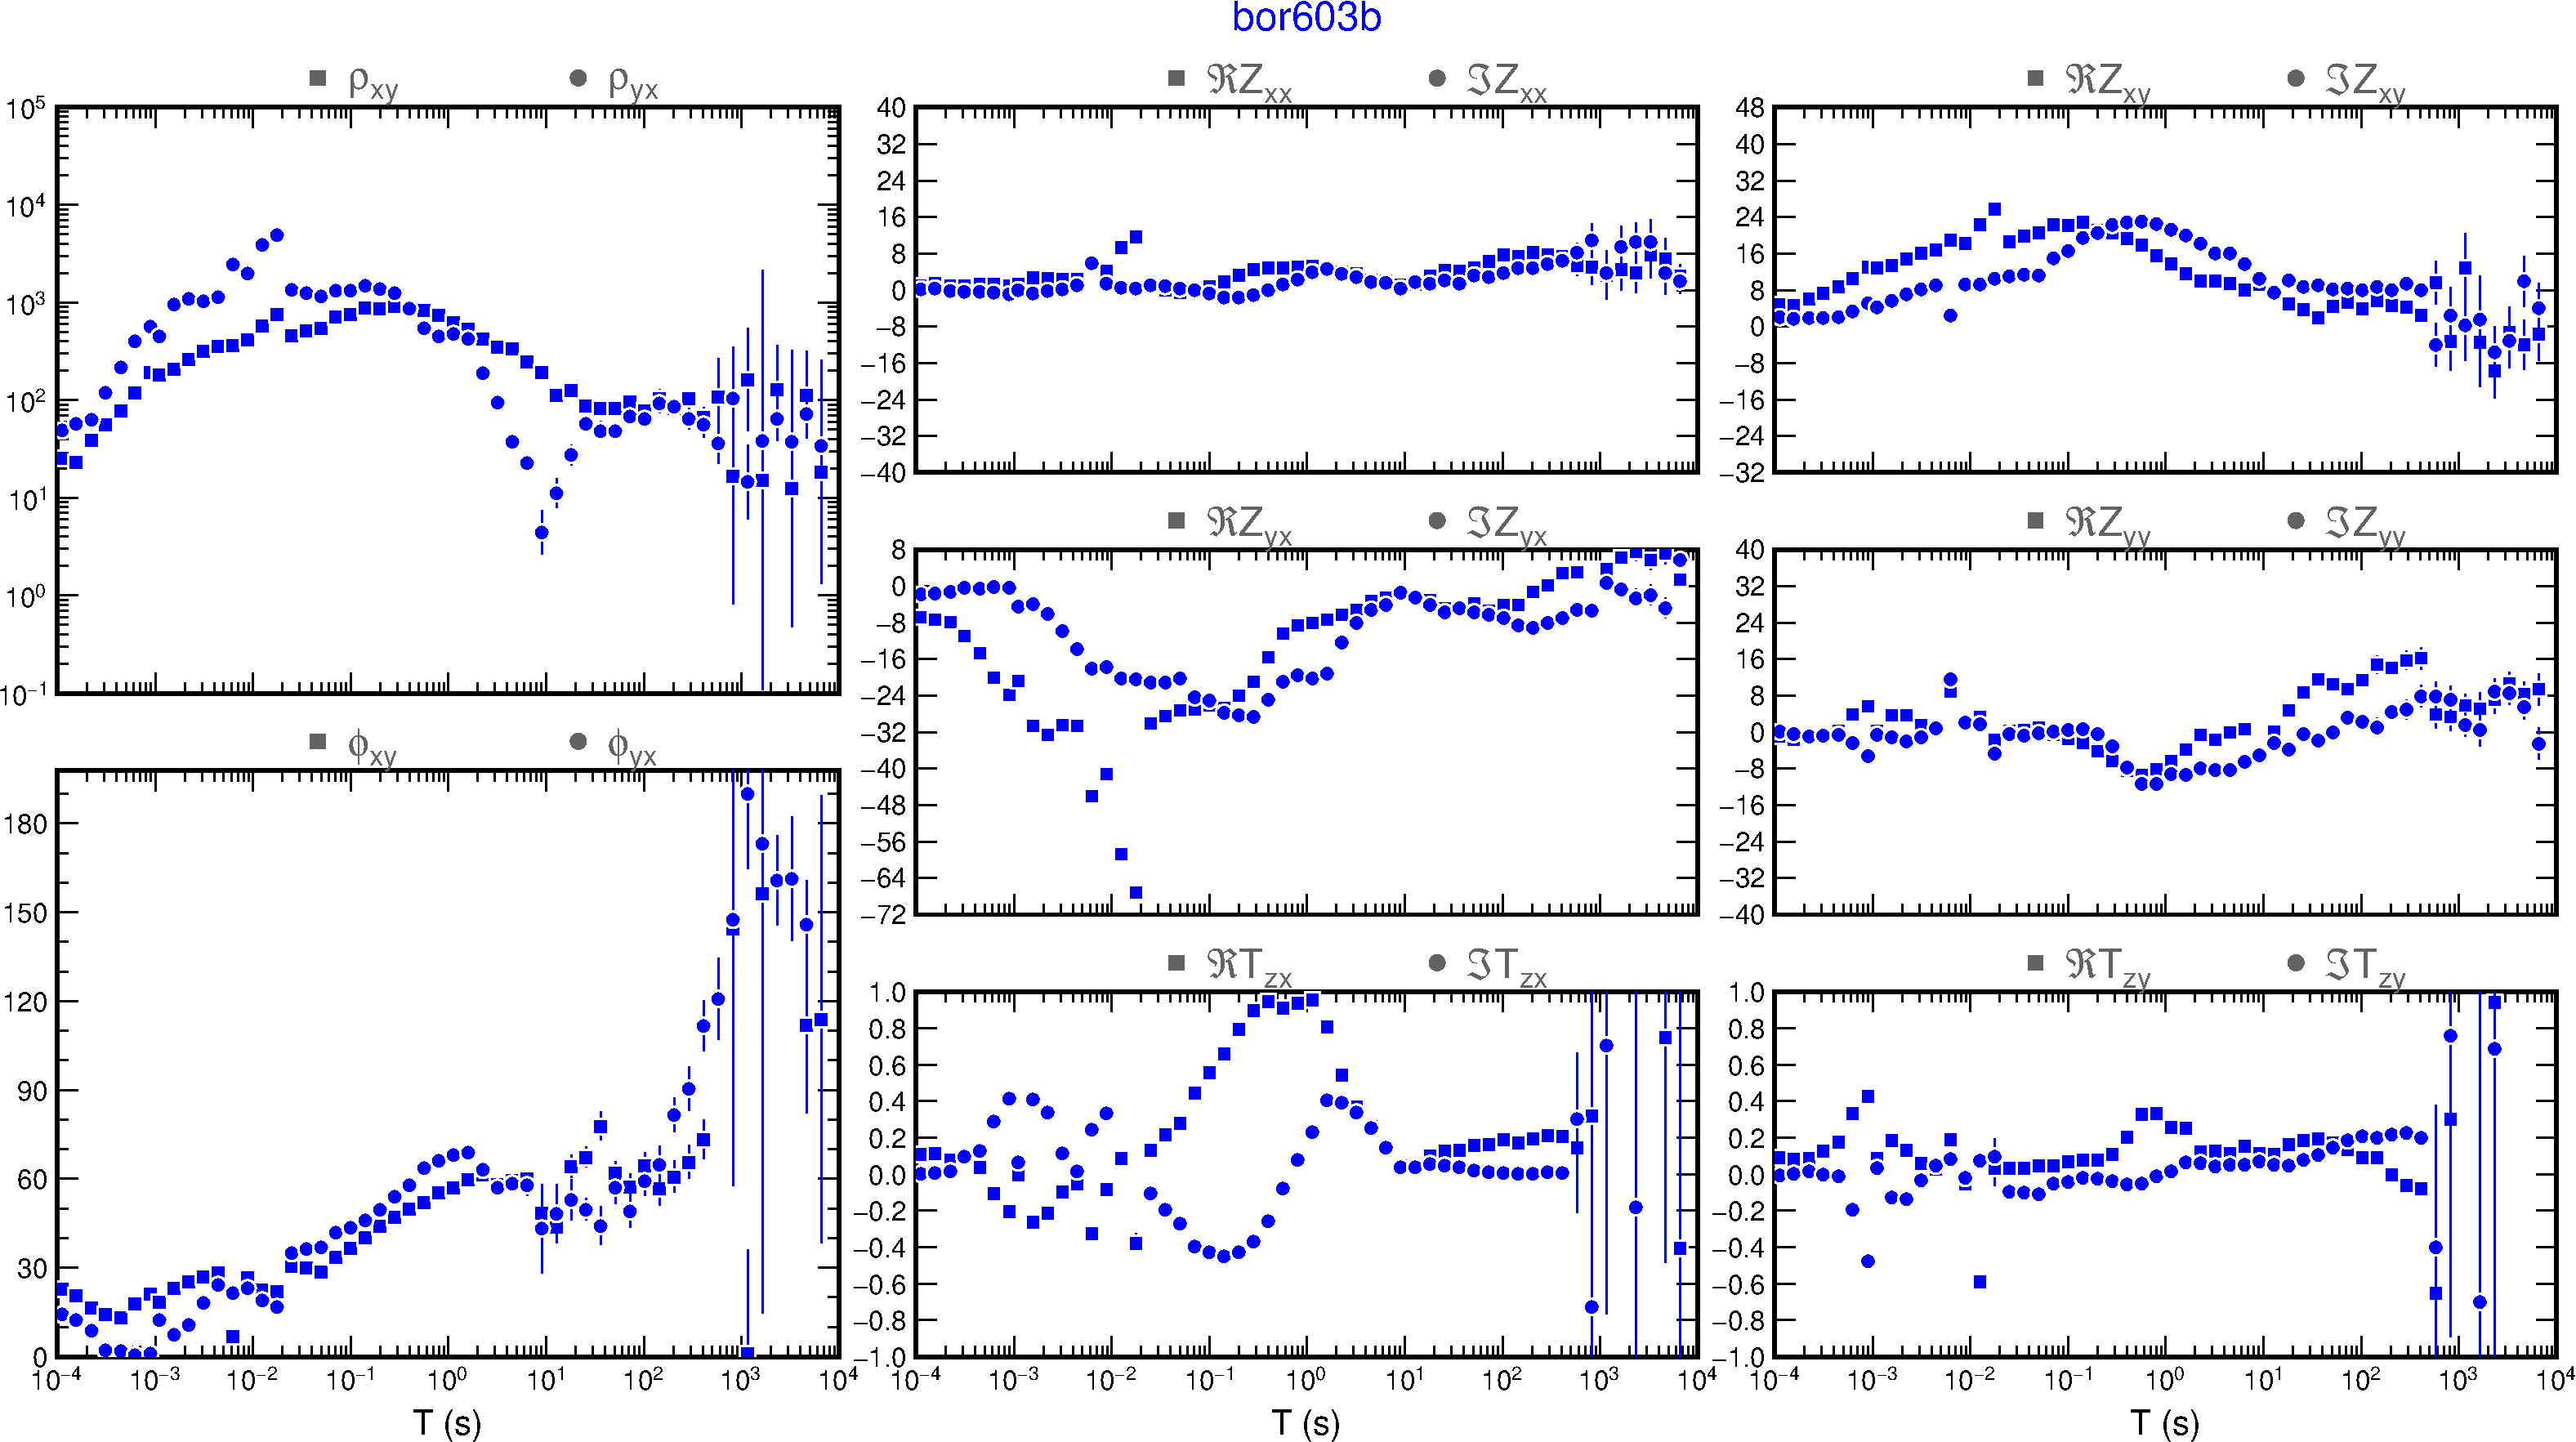
\includegraphics[width=15cm]{texto/figura/sites/M-bor603b.png}
            \end{center}
        \legend{\Fonte{\oautor.}}
    \end{figure}
    %\end{landscape}
    \begin{figure}[H]
        \caption{Manual -- bor604a}
            \begin{center}
                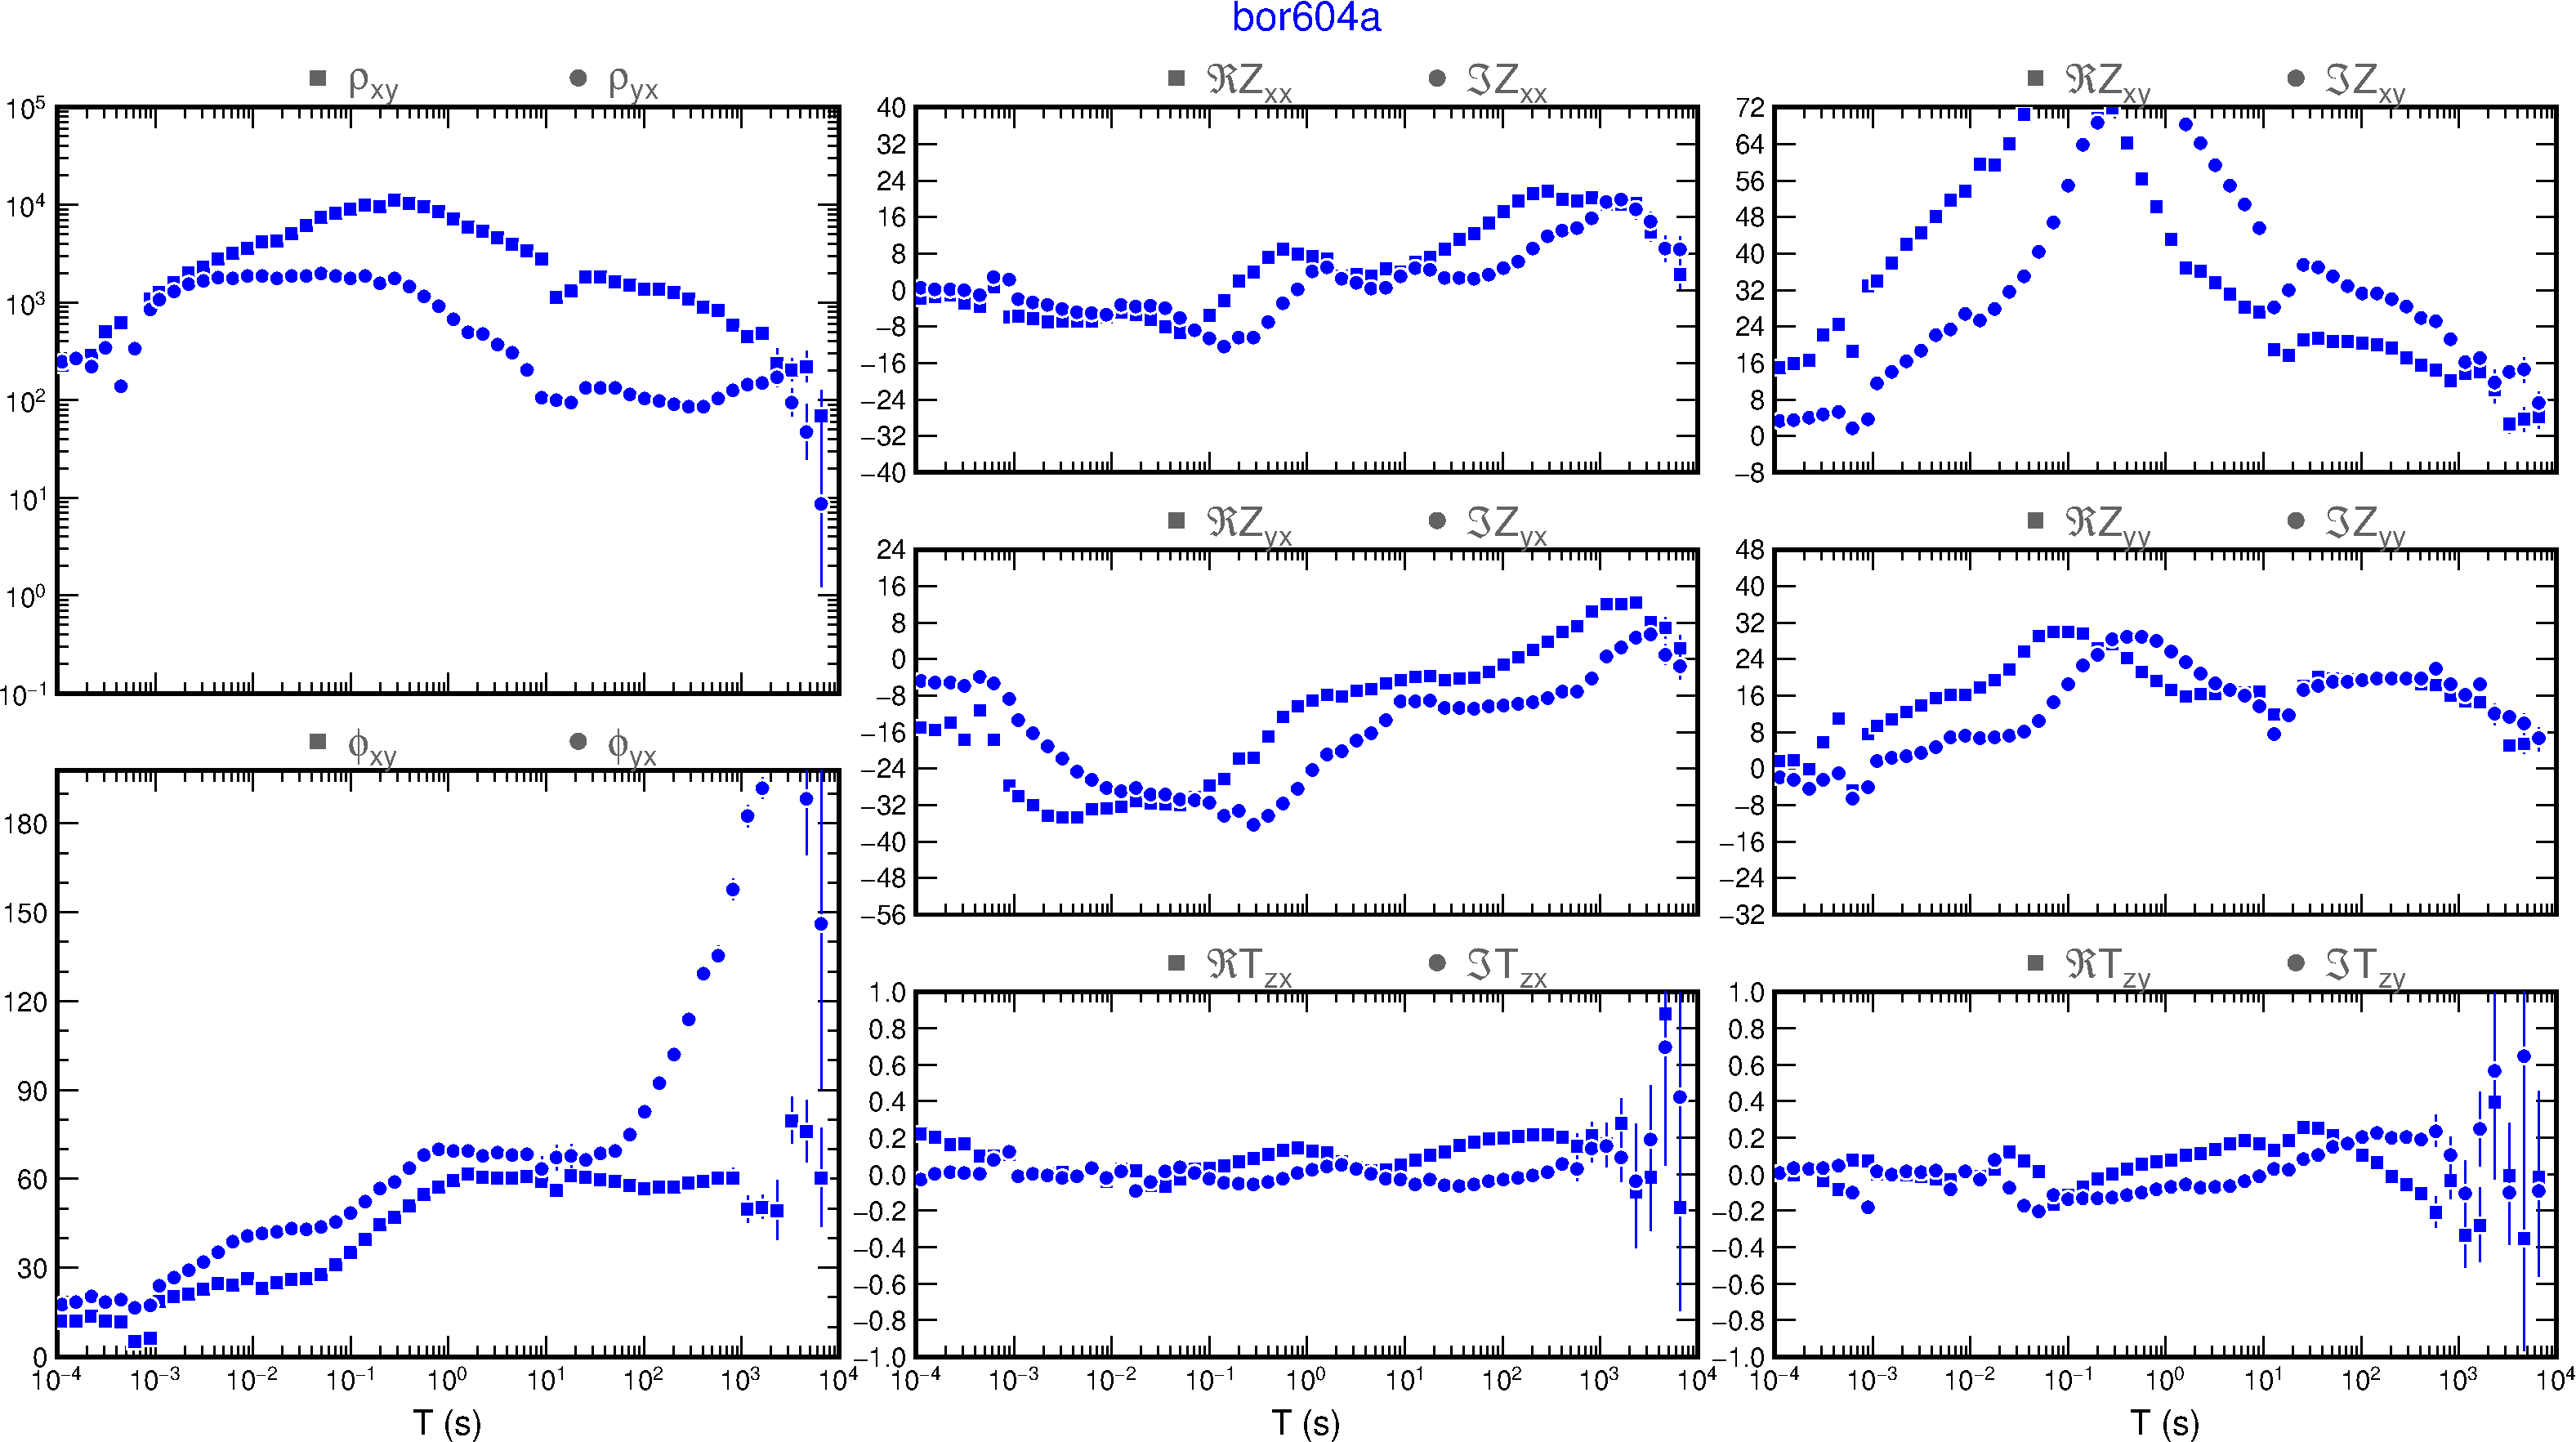
\includegraphics[width=15cm]{texto/figura/sites/M-bor604a.png}
            \end{center}
        \legend{\Fonte{\oautor.}}
    \end{figure}
    
    \begin{figure}[H]
        \caption{Manual -- bor604b}
            \begin{center}
                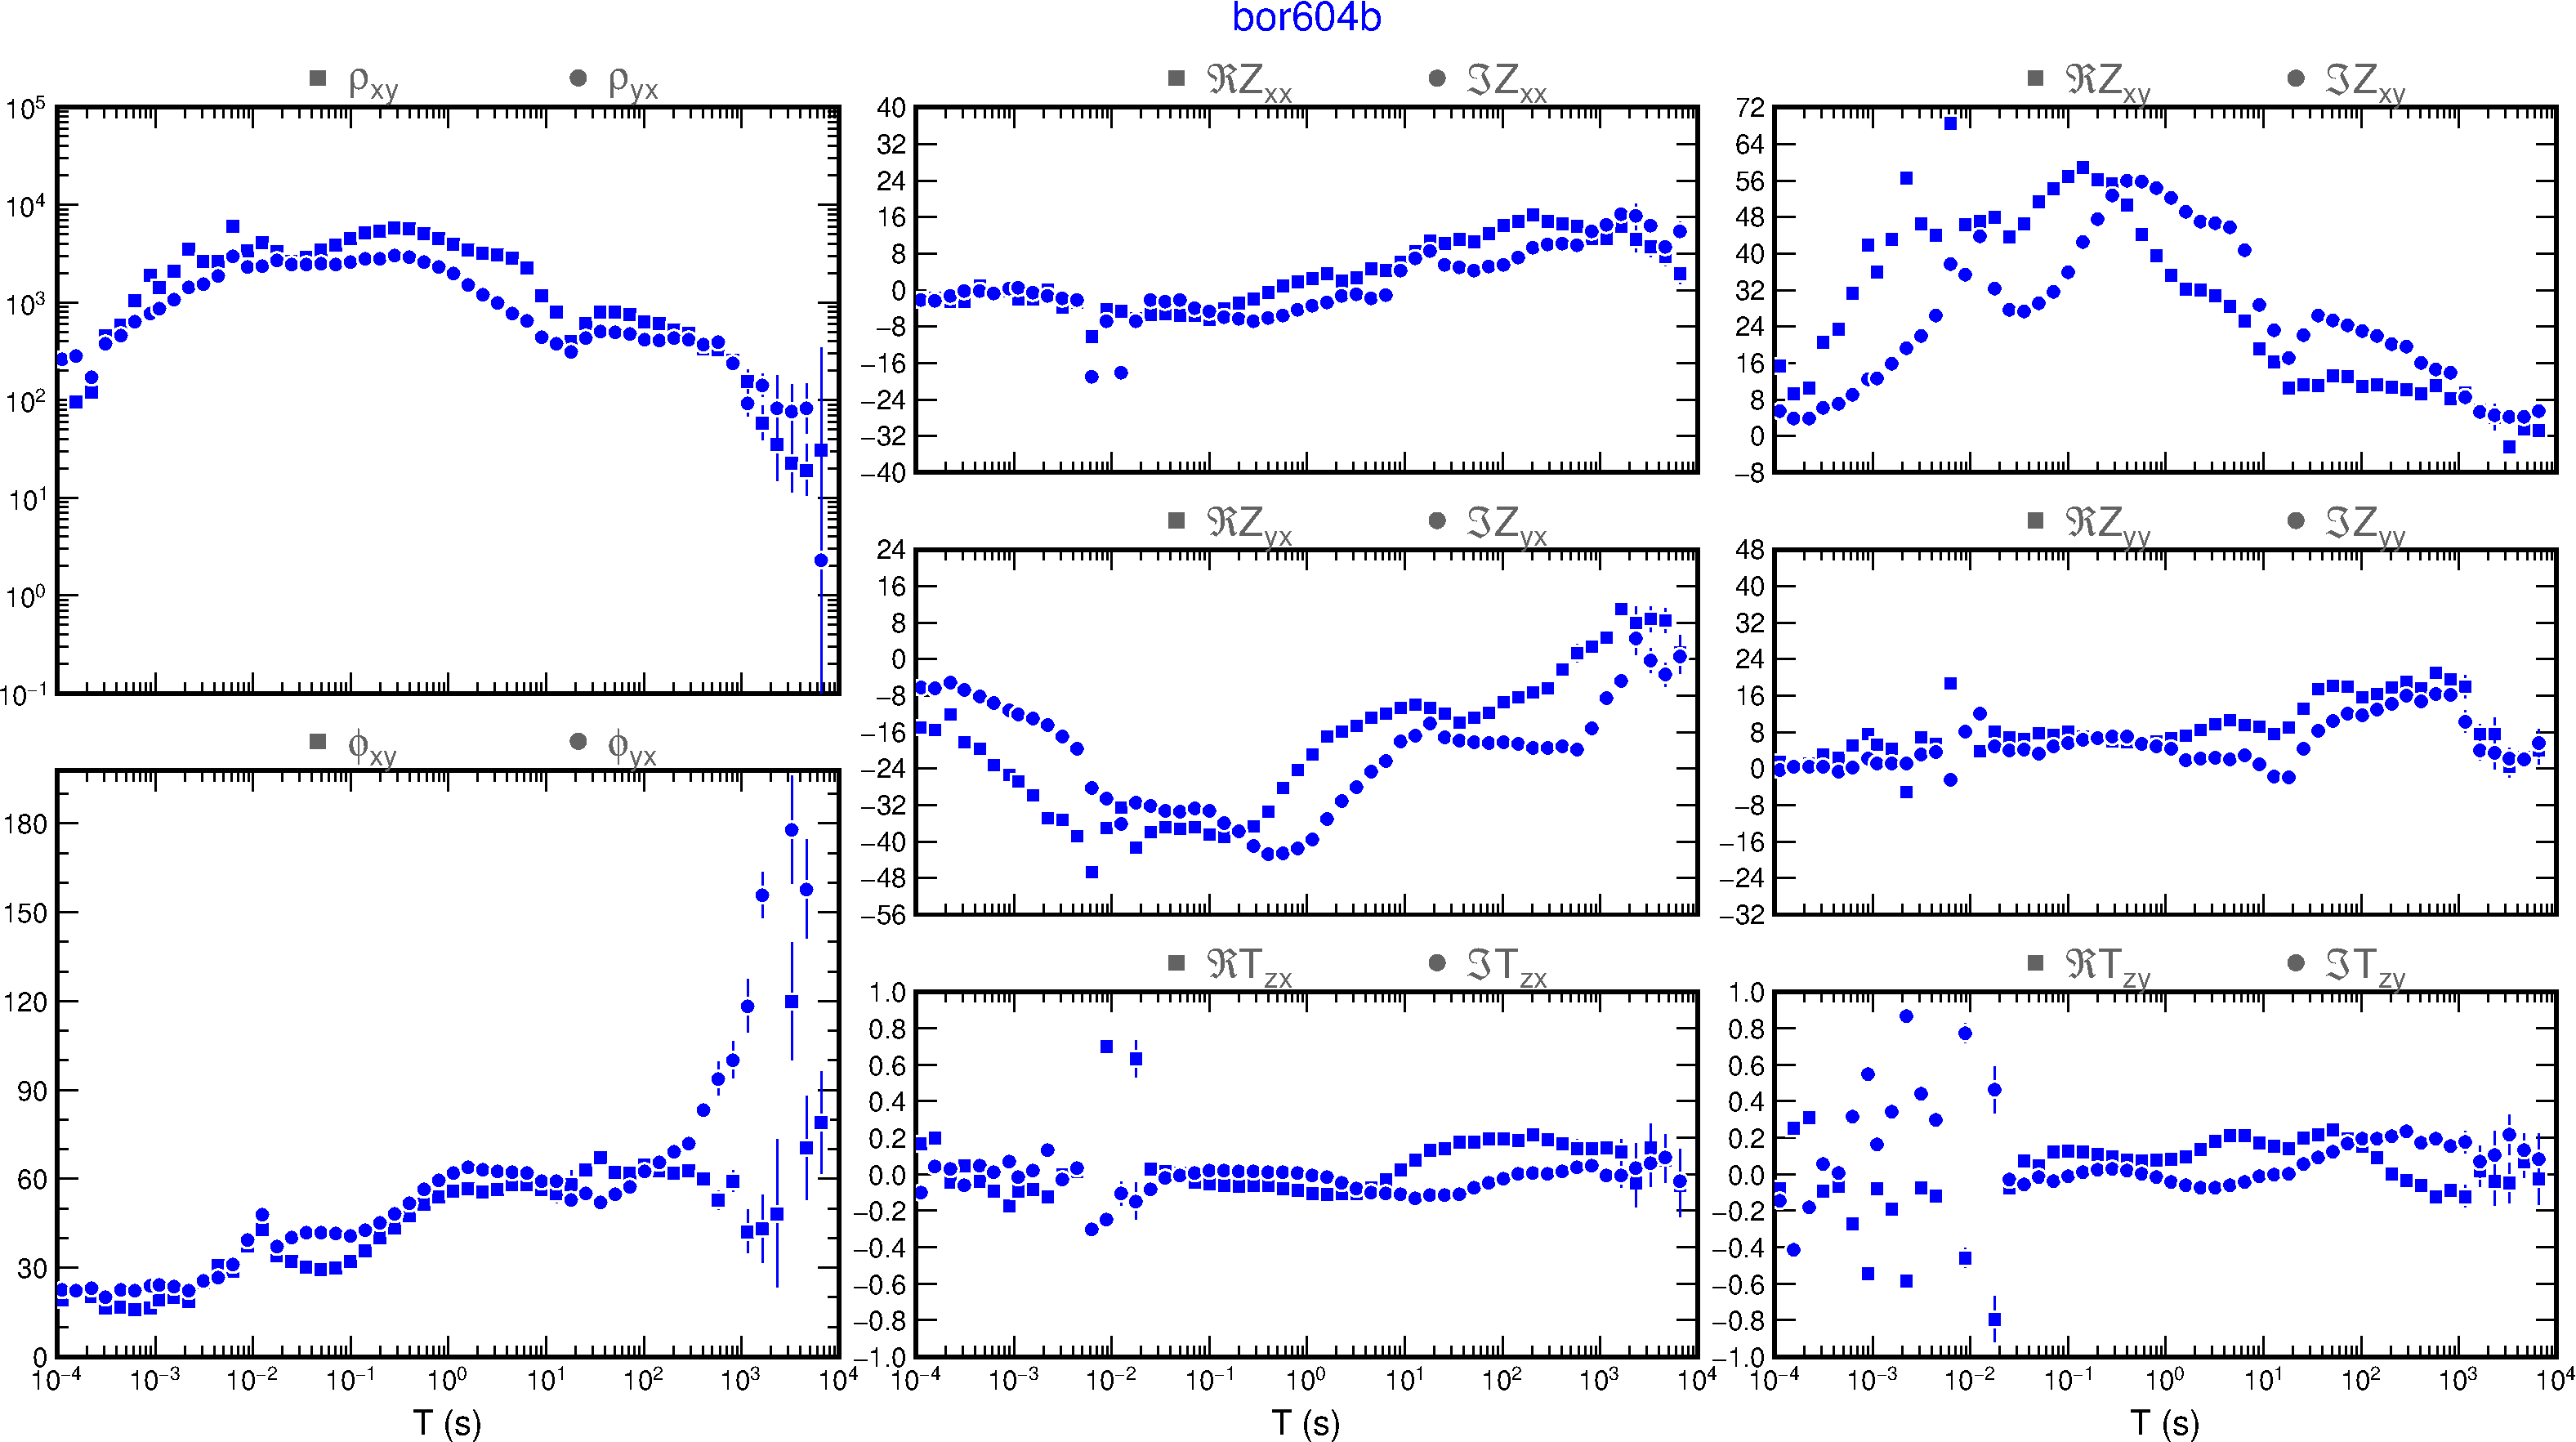
\includegraphics[width=16cm]{texto/figura/sites/M-bor604b.png}
            \end{center}
        \legend{\Fonte{\oautor.}}
    \end{figure}
    
    \begin{figure}[H]
        \caption{Manual -- bor605a}
            \begin{center}
                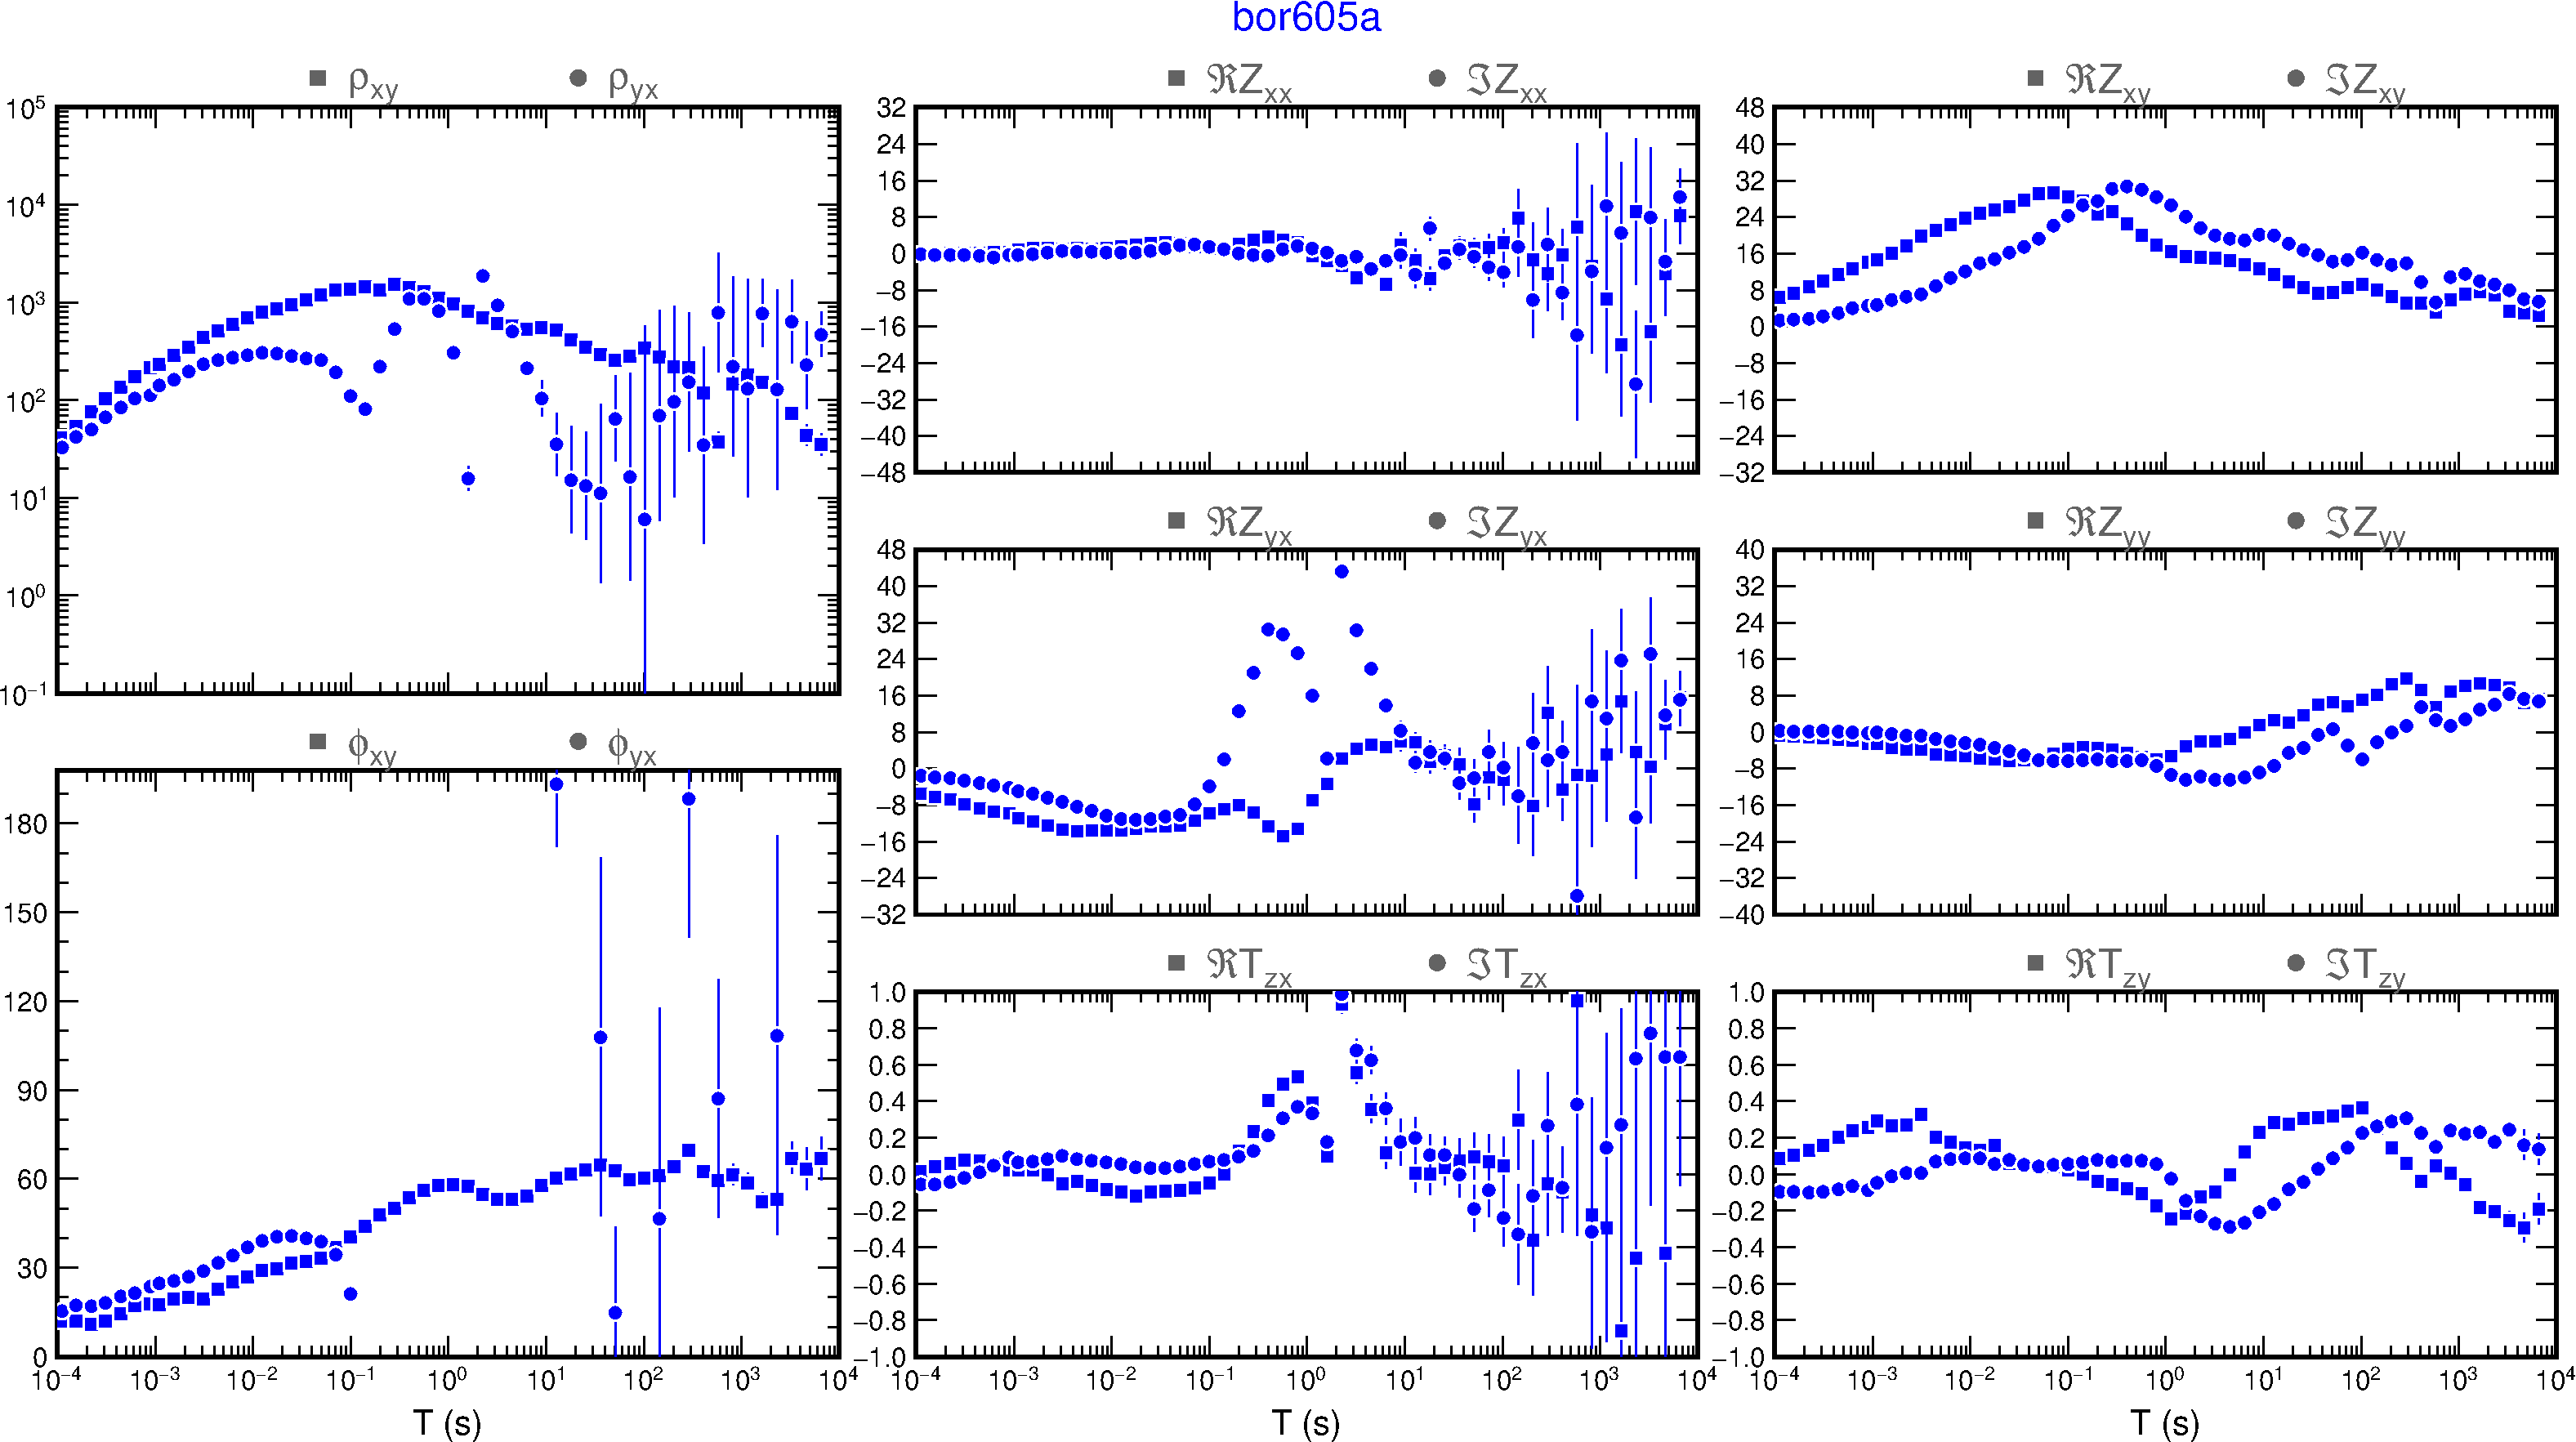
\includegraphics[width=16cm]{texto/figura/sites/M-bor605a.png}
            \end{center}
        \legend{\Fonte{\oautor.}}
    \end{figure}
    
    \begin{figure}[H]
        \caption{Manual -- bor605b}
            \begin{center}
                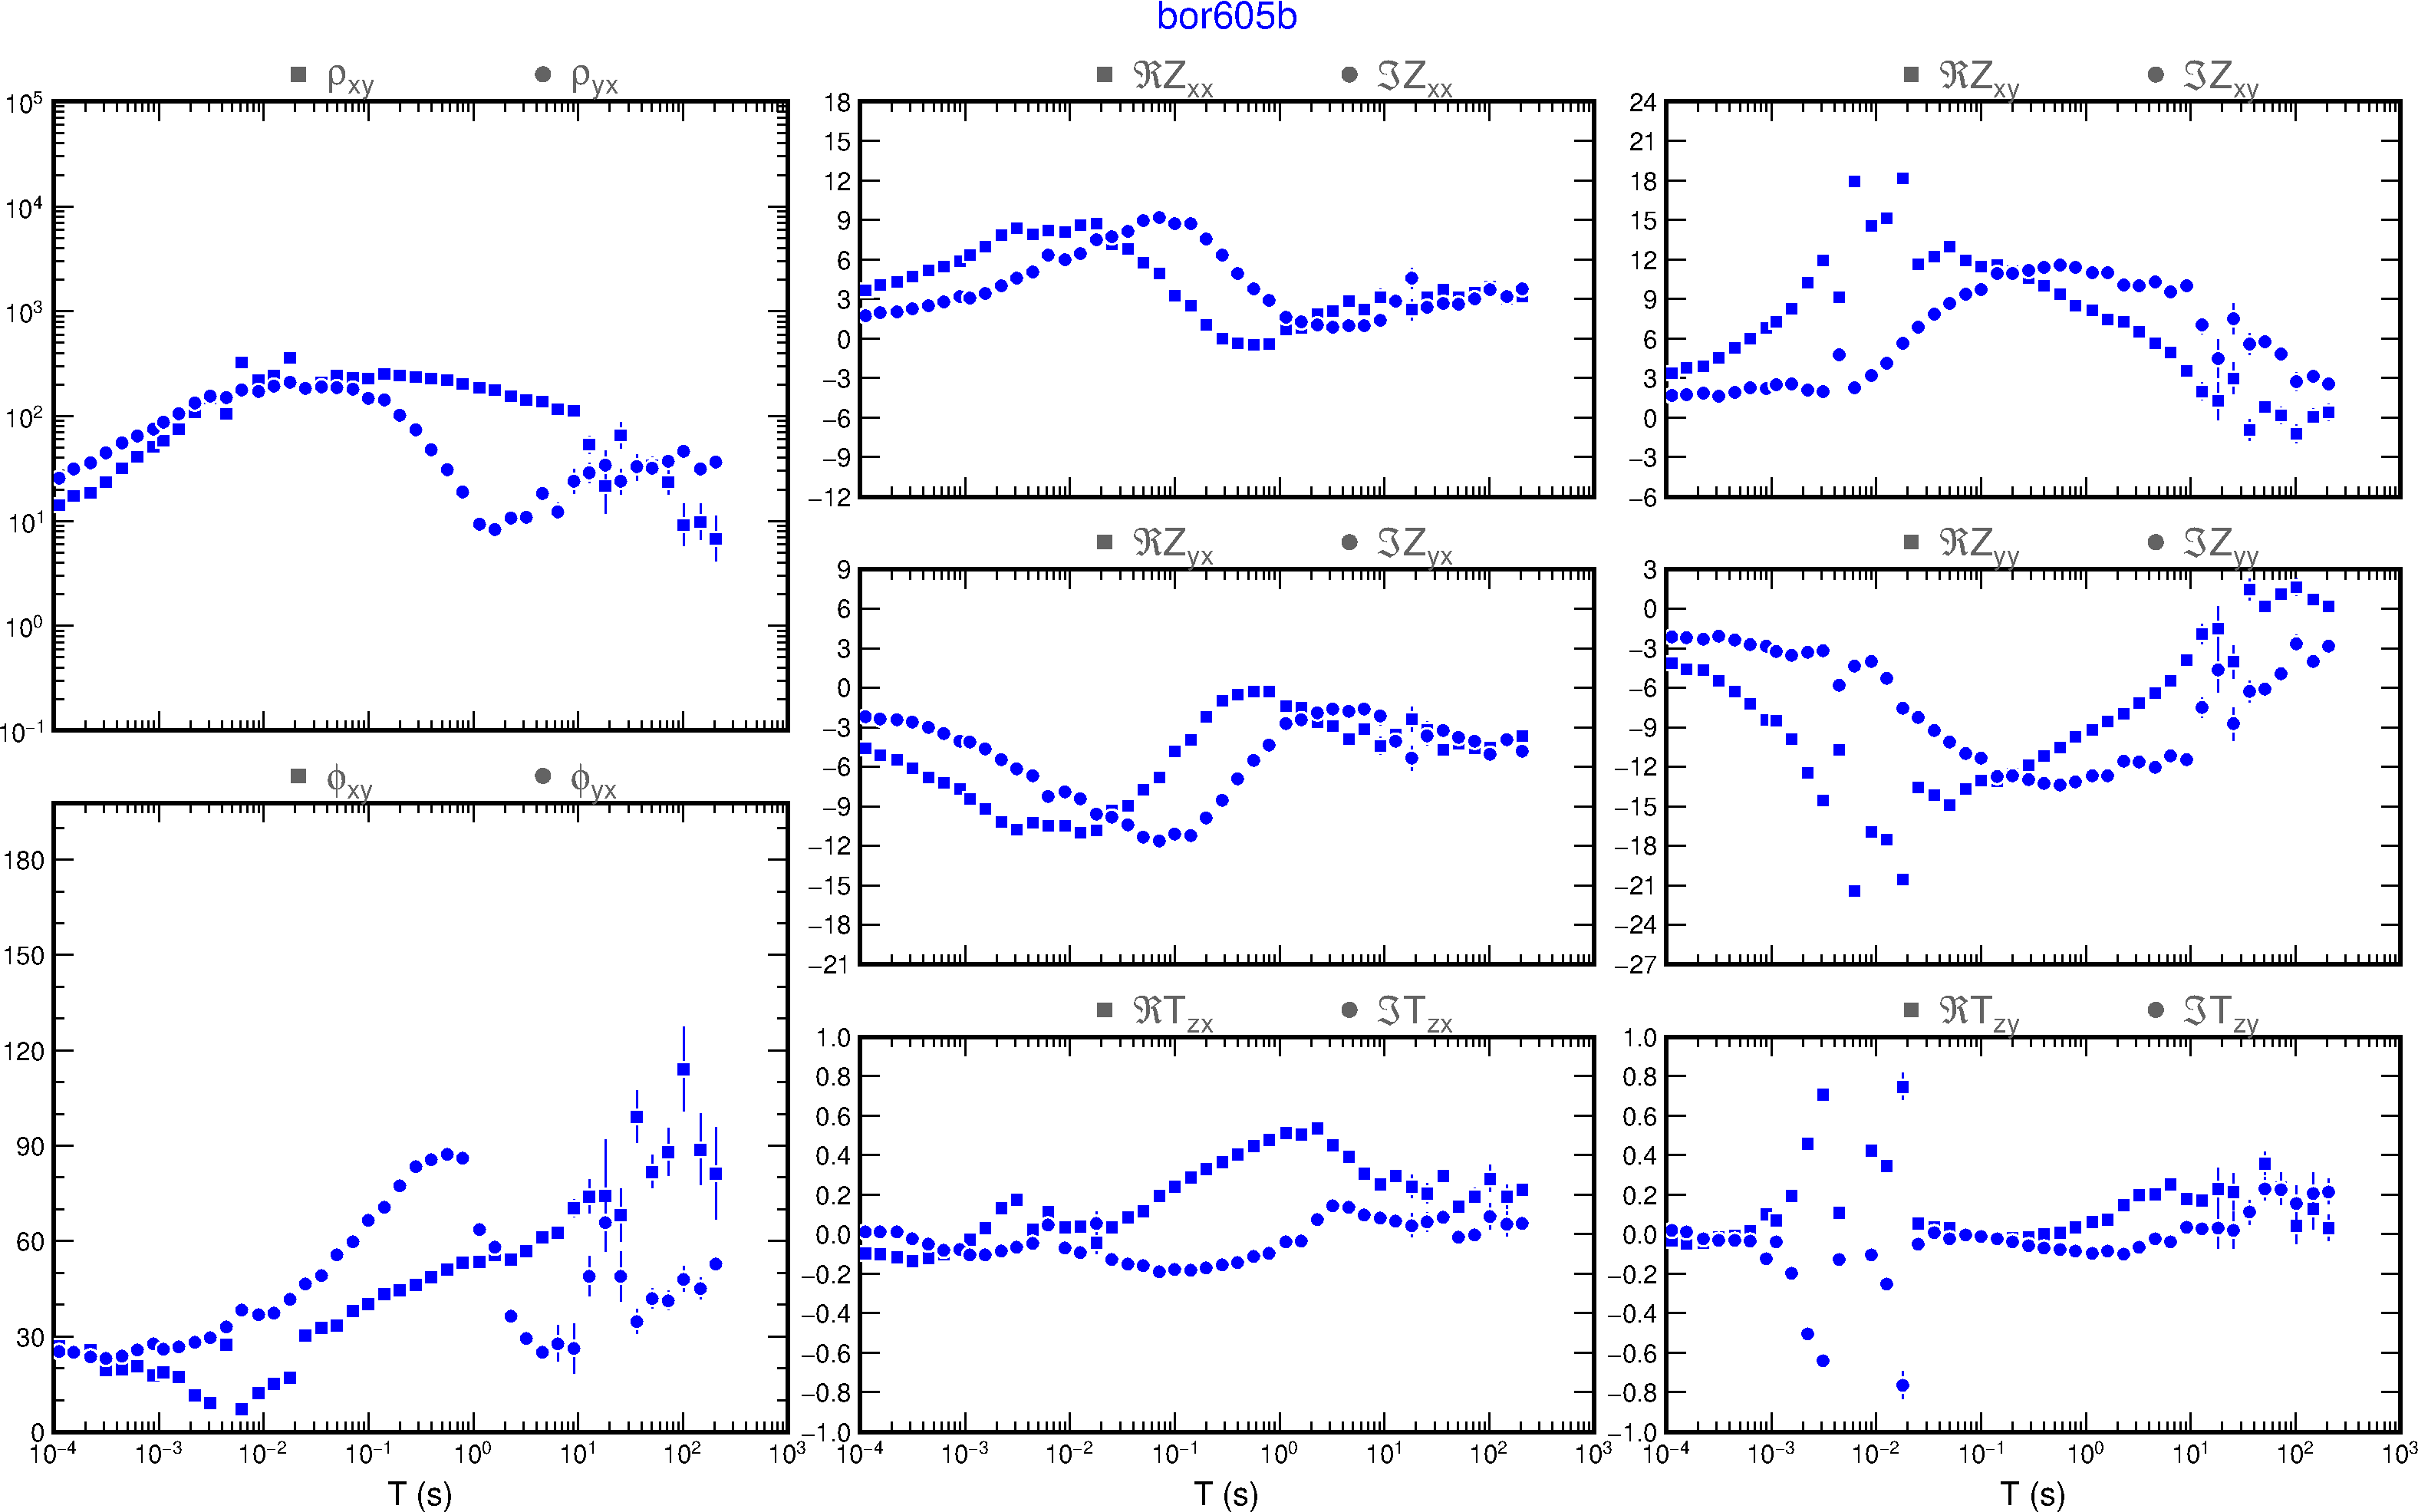
\includegraphics[width=15cm]{texto/figura/sites/M-bor605b.png}
            \end{center}
        \legend{\Fonte{\oautor.}}
    \end{figure}
    
    \begin{figure}[H]
        \caption{Manual -- bor606a}
            \begin{center}
                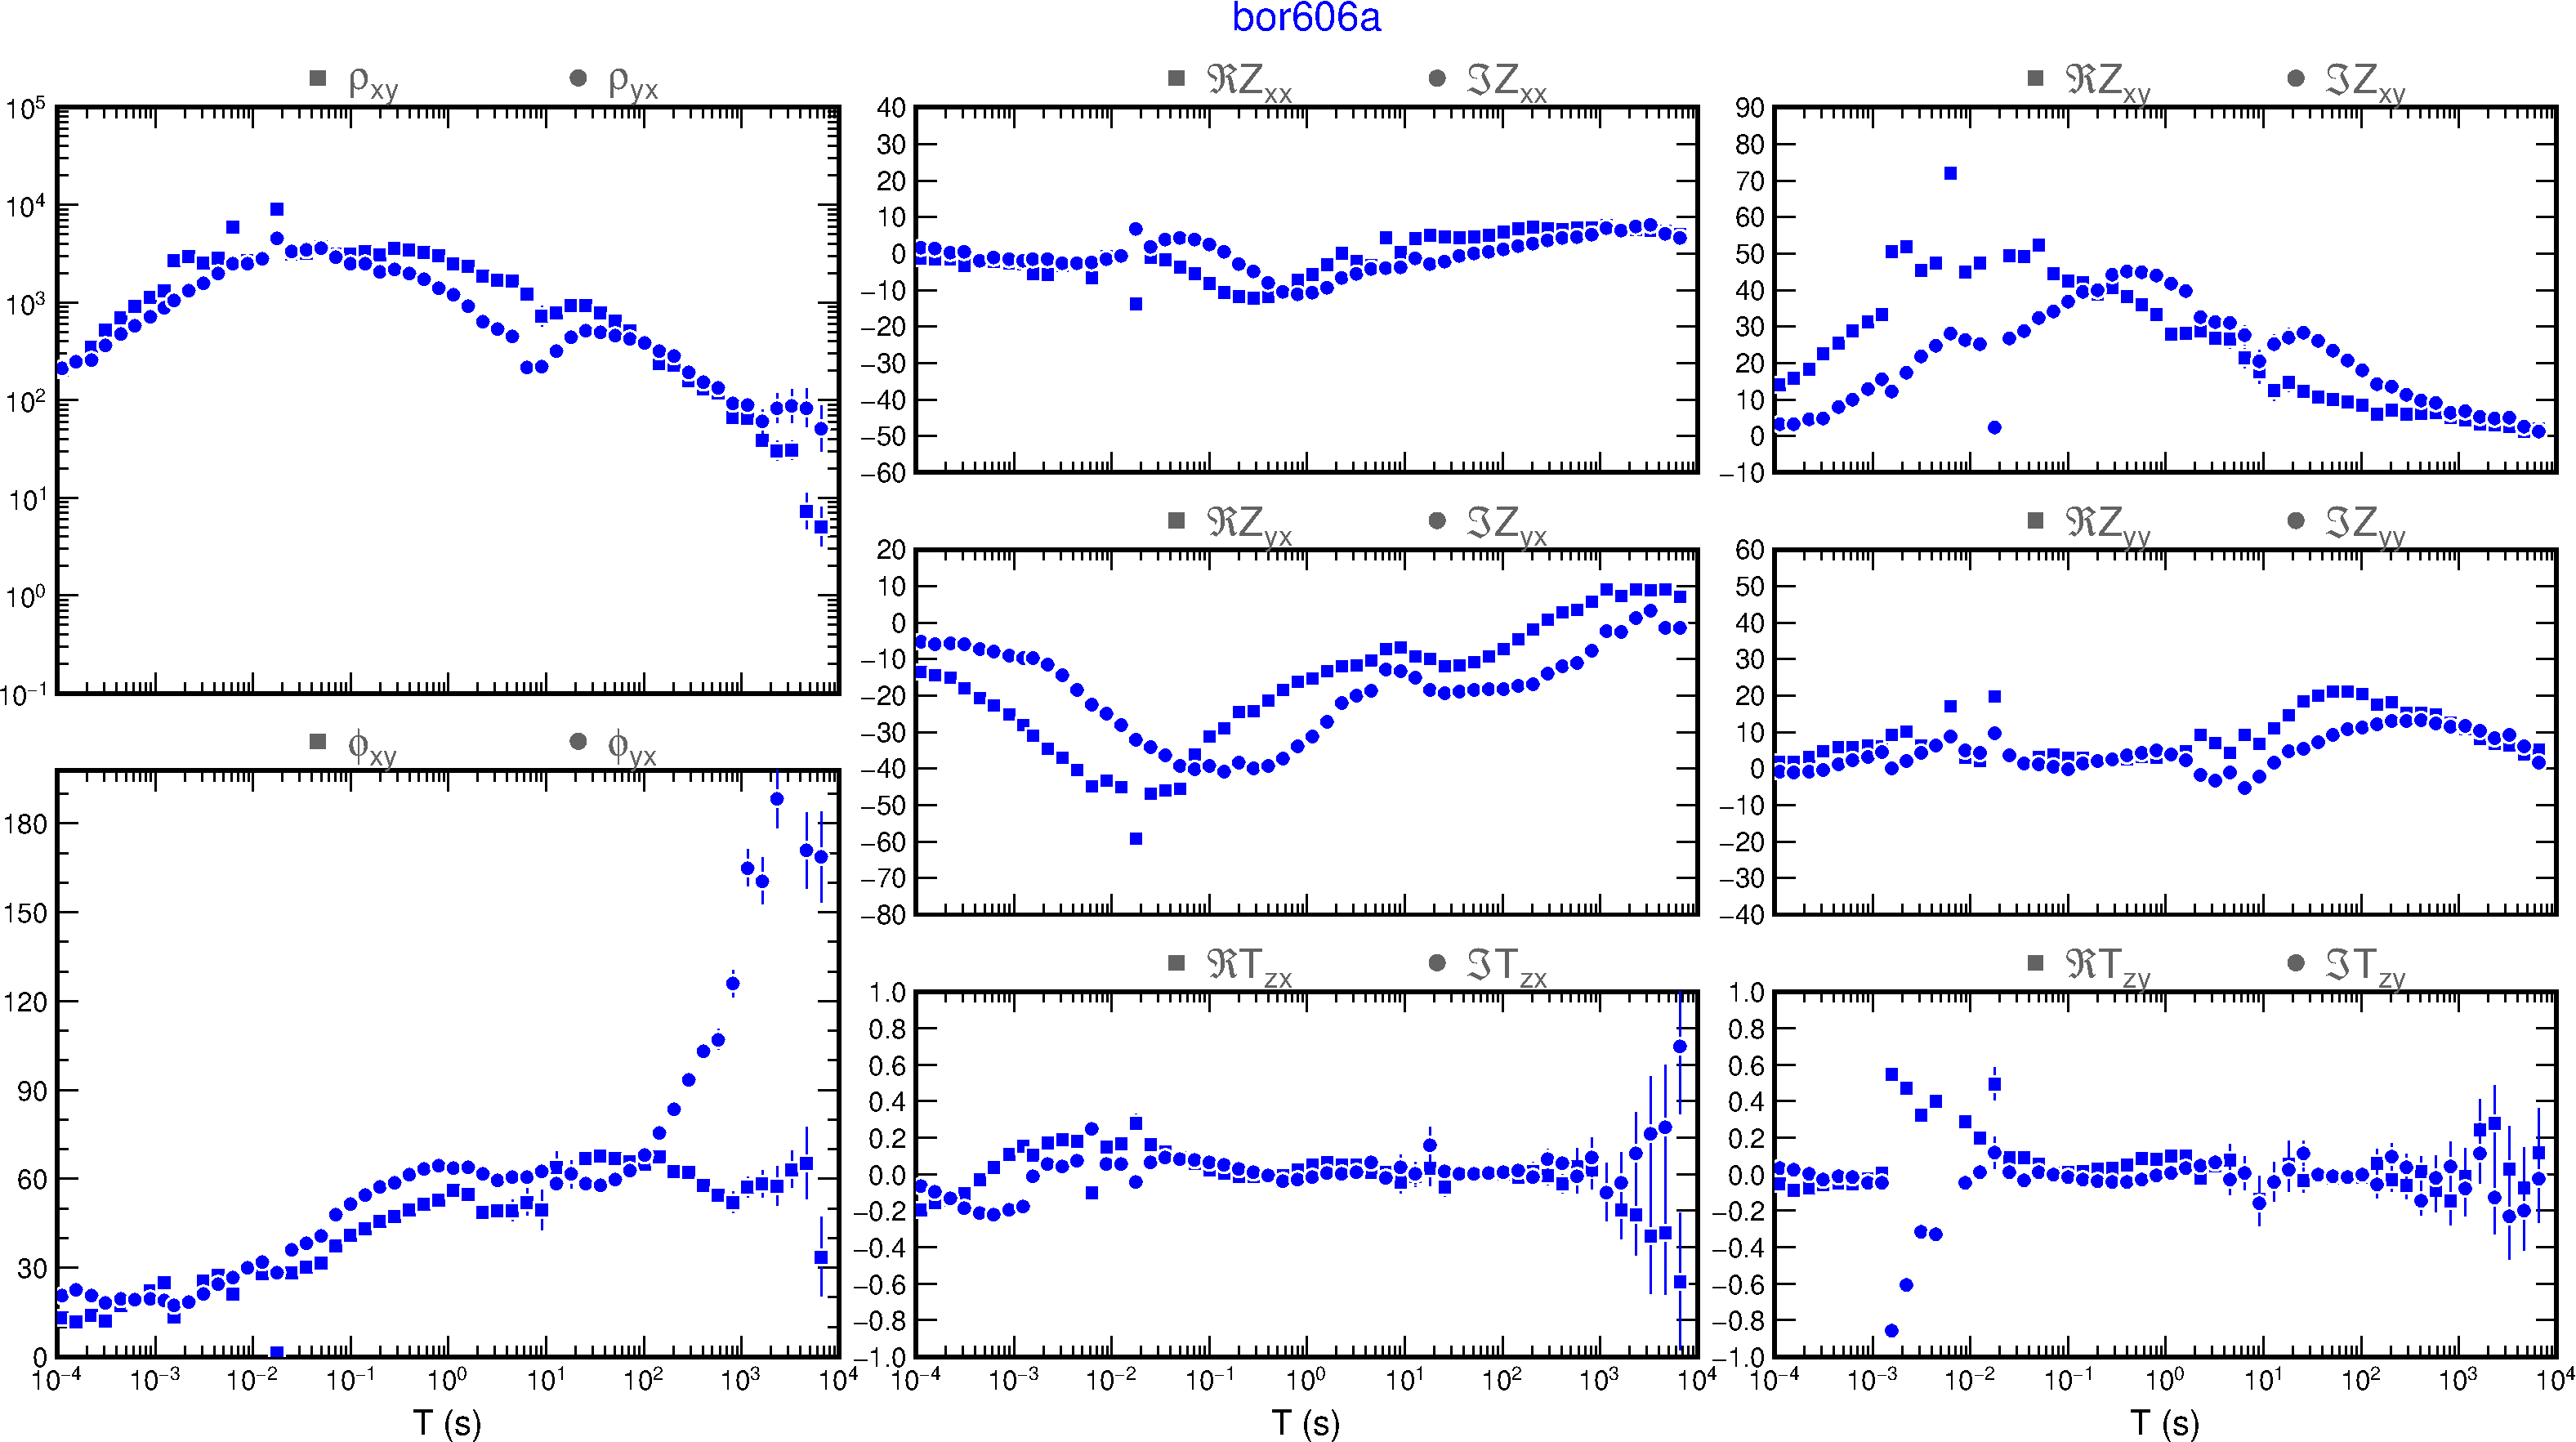
\includegraphics[width=15cm]{texto/figura/sites/M-bor606a.png}
            \end{center}
        \legend{\Fonte{\oautor.}}
    \end{figure}
    
    \begin{figure}[H]
        \caption{Manual -- bor606b}
            \begin{center}
                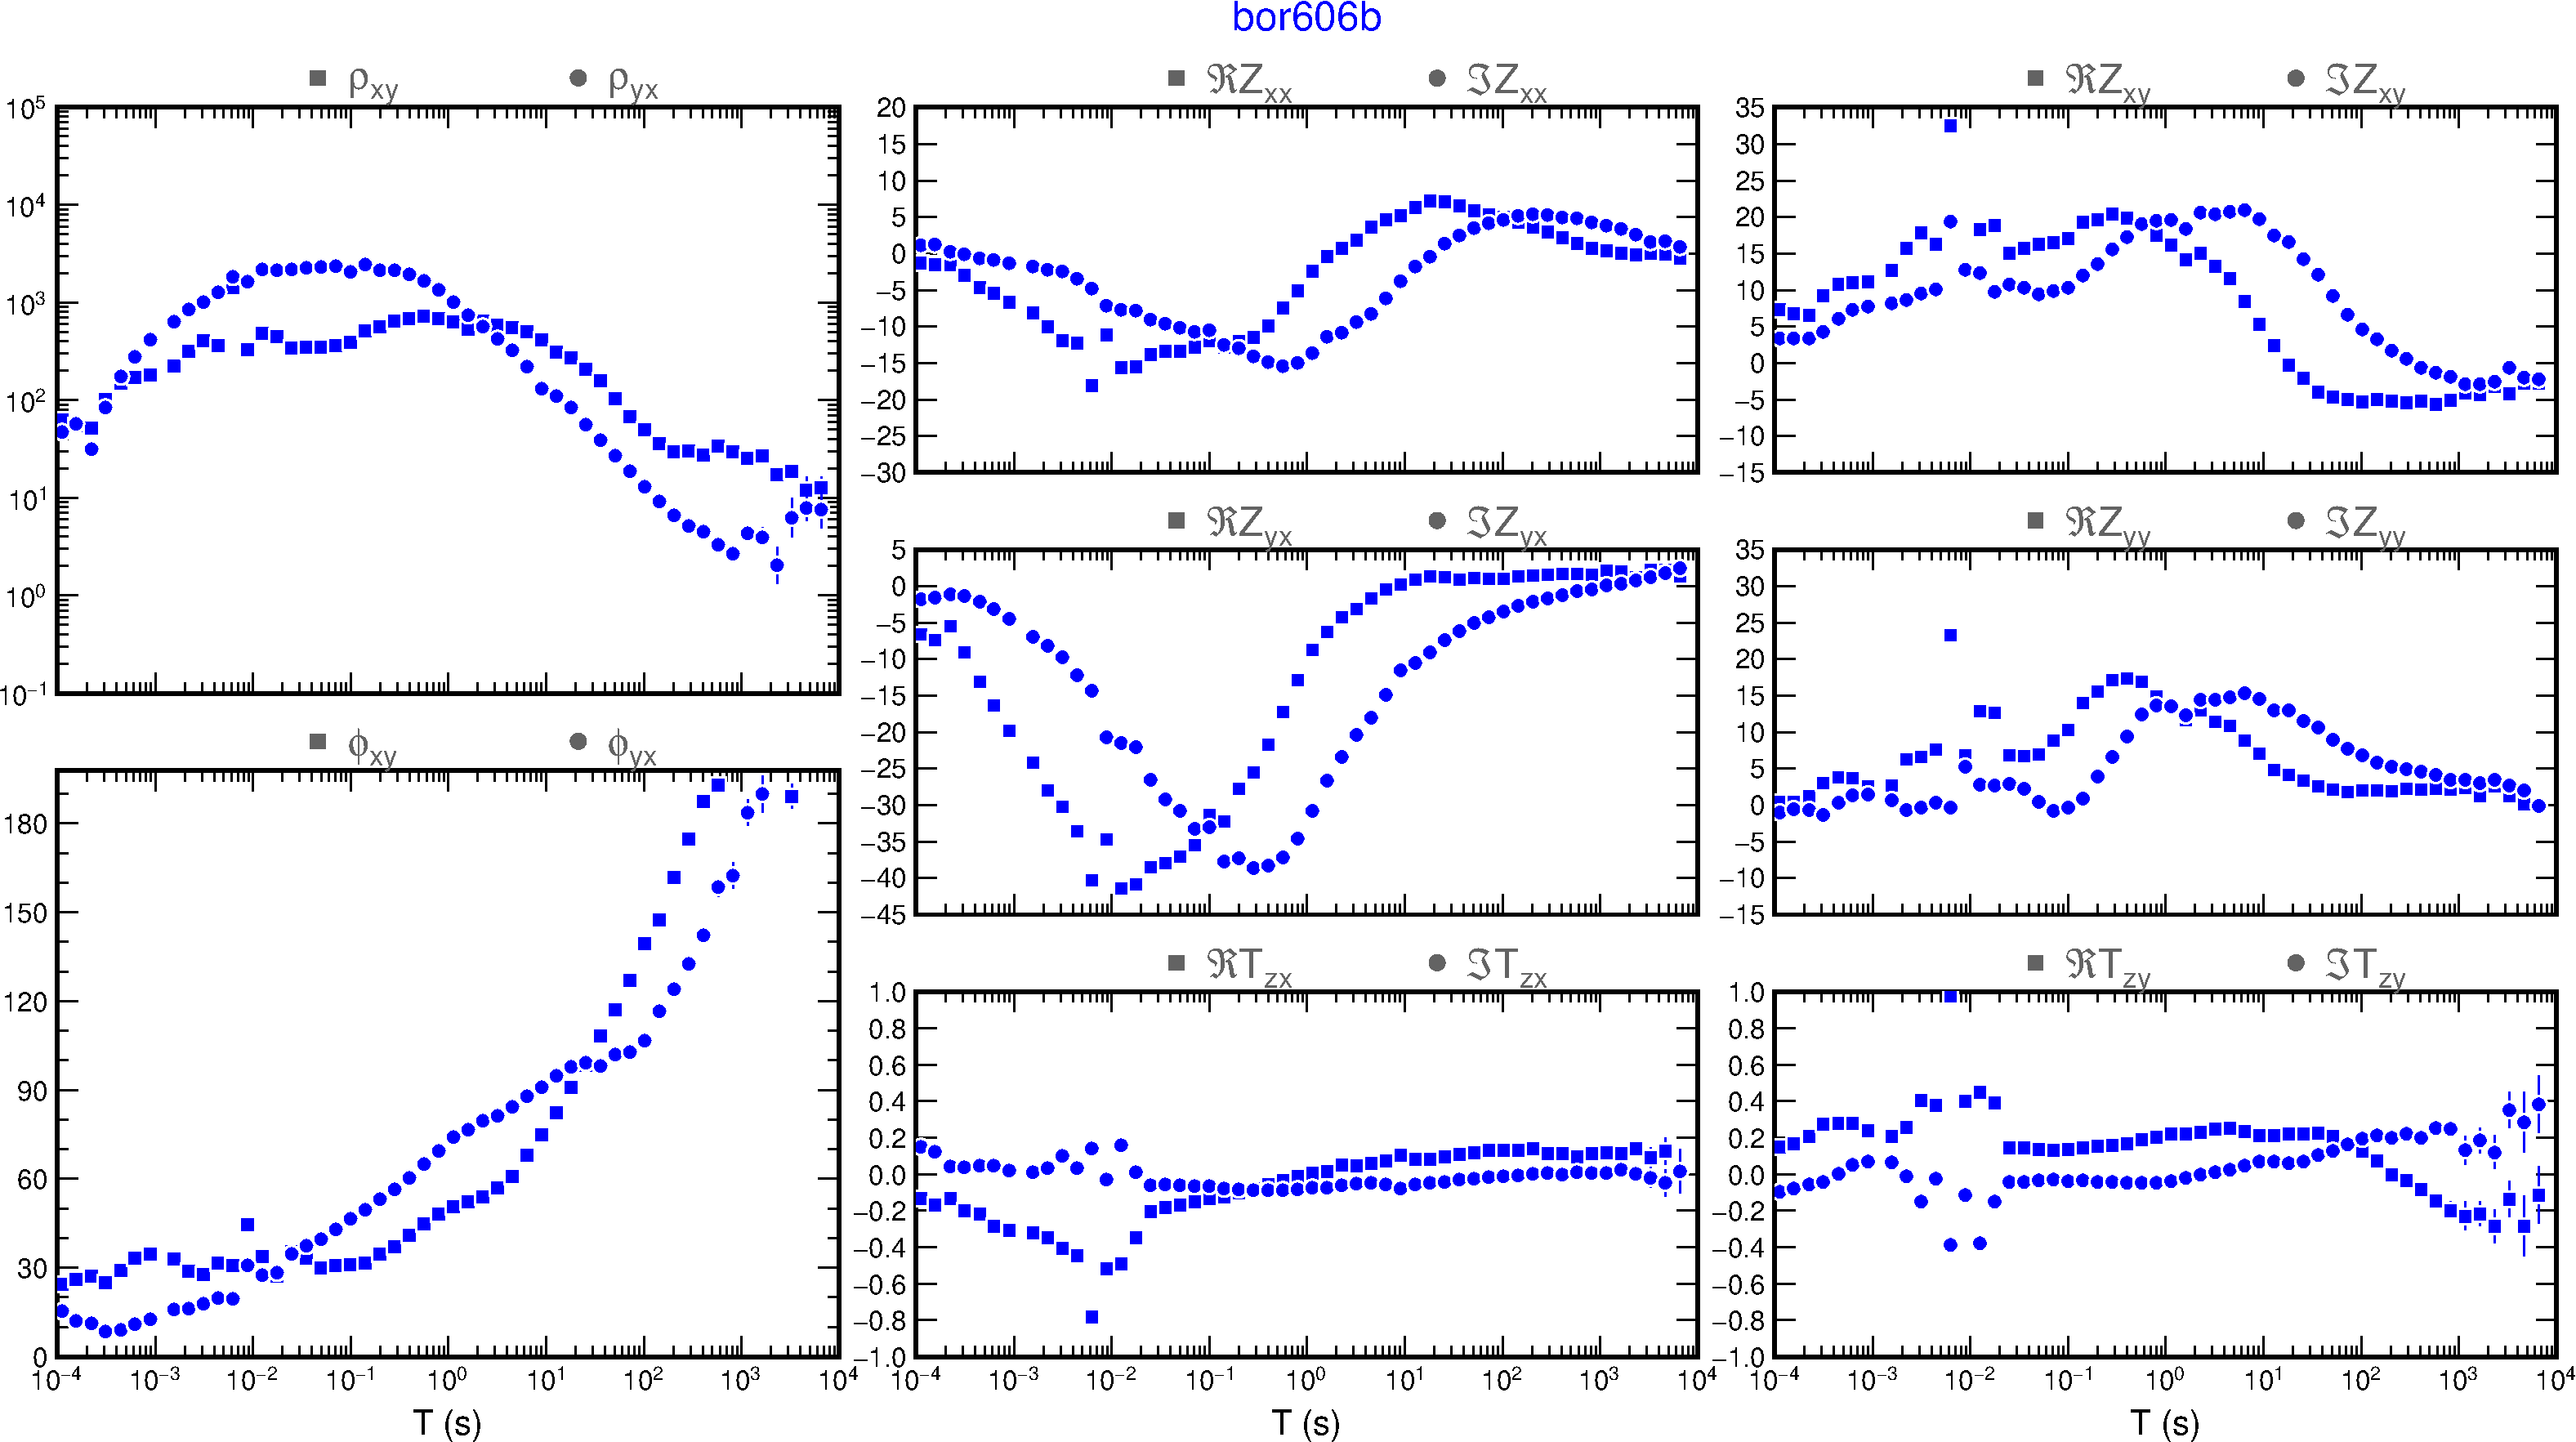
\includegraphics[width=16cm]{texto/figura/sites/M-bor606b.png}
            \end{center}
        \legend{\Fonte{\oautor.}}
    \end{figure}
    
    \begin{figure}[H]
        \caption{Manual -- bor607a}
            \begin{center}
                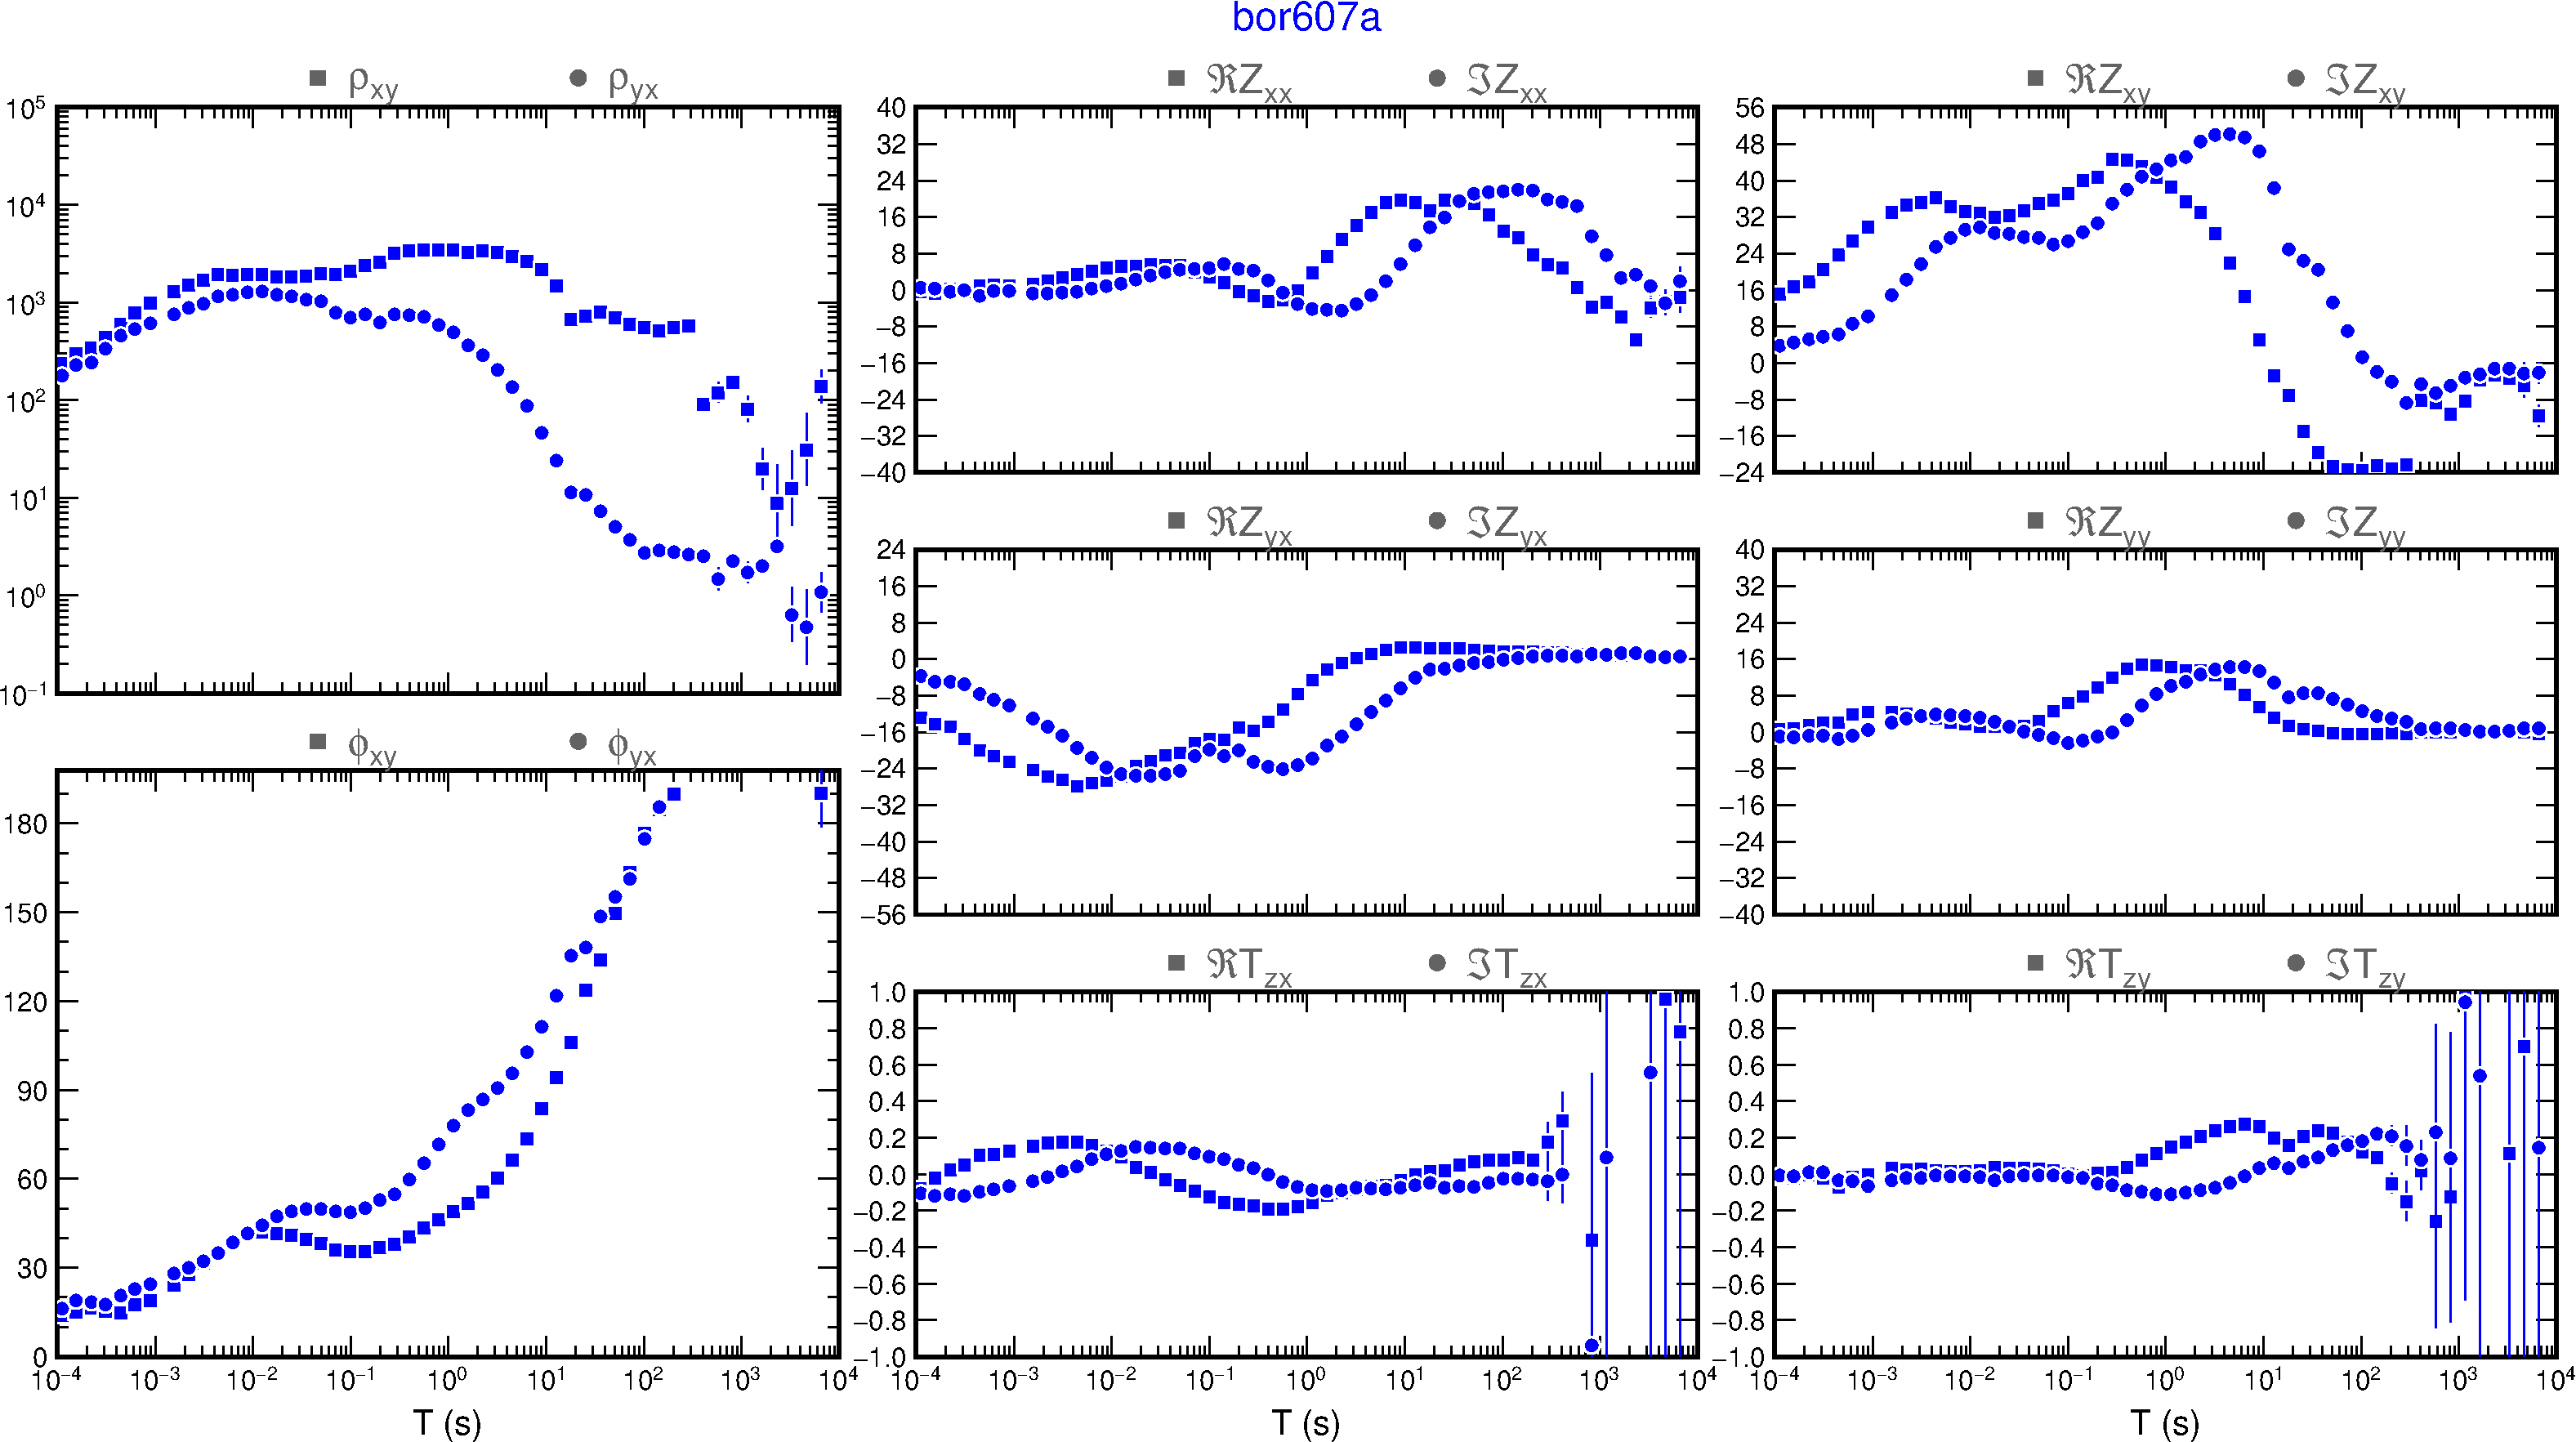
\includegraphics[width=16cm]{texto/figura/sites/M-bor607a.png}
            \end{center}
        \legend{\Fonte{\oautor.}}
    \end{figure}
    
    \begin{figure}[H]
        \caption{Manual -- bor607b}
            \begin{center}
                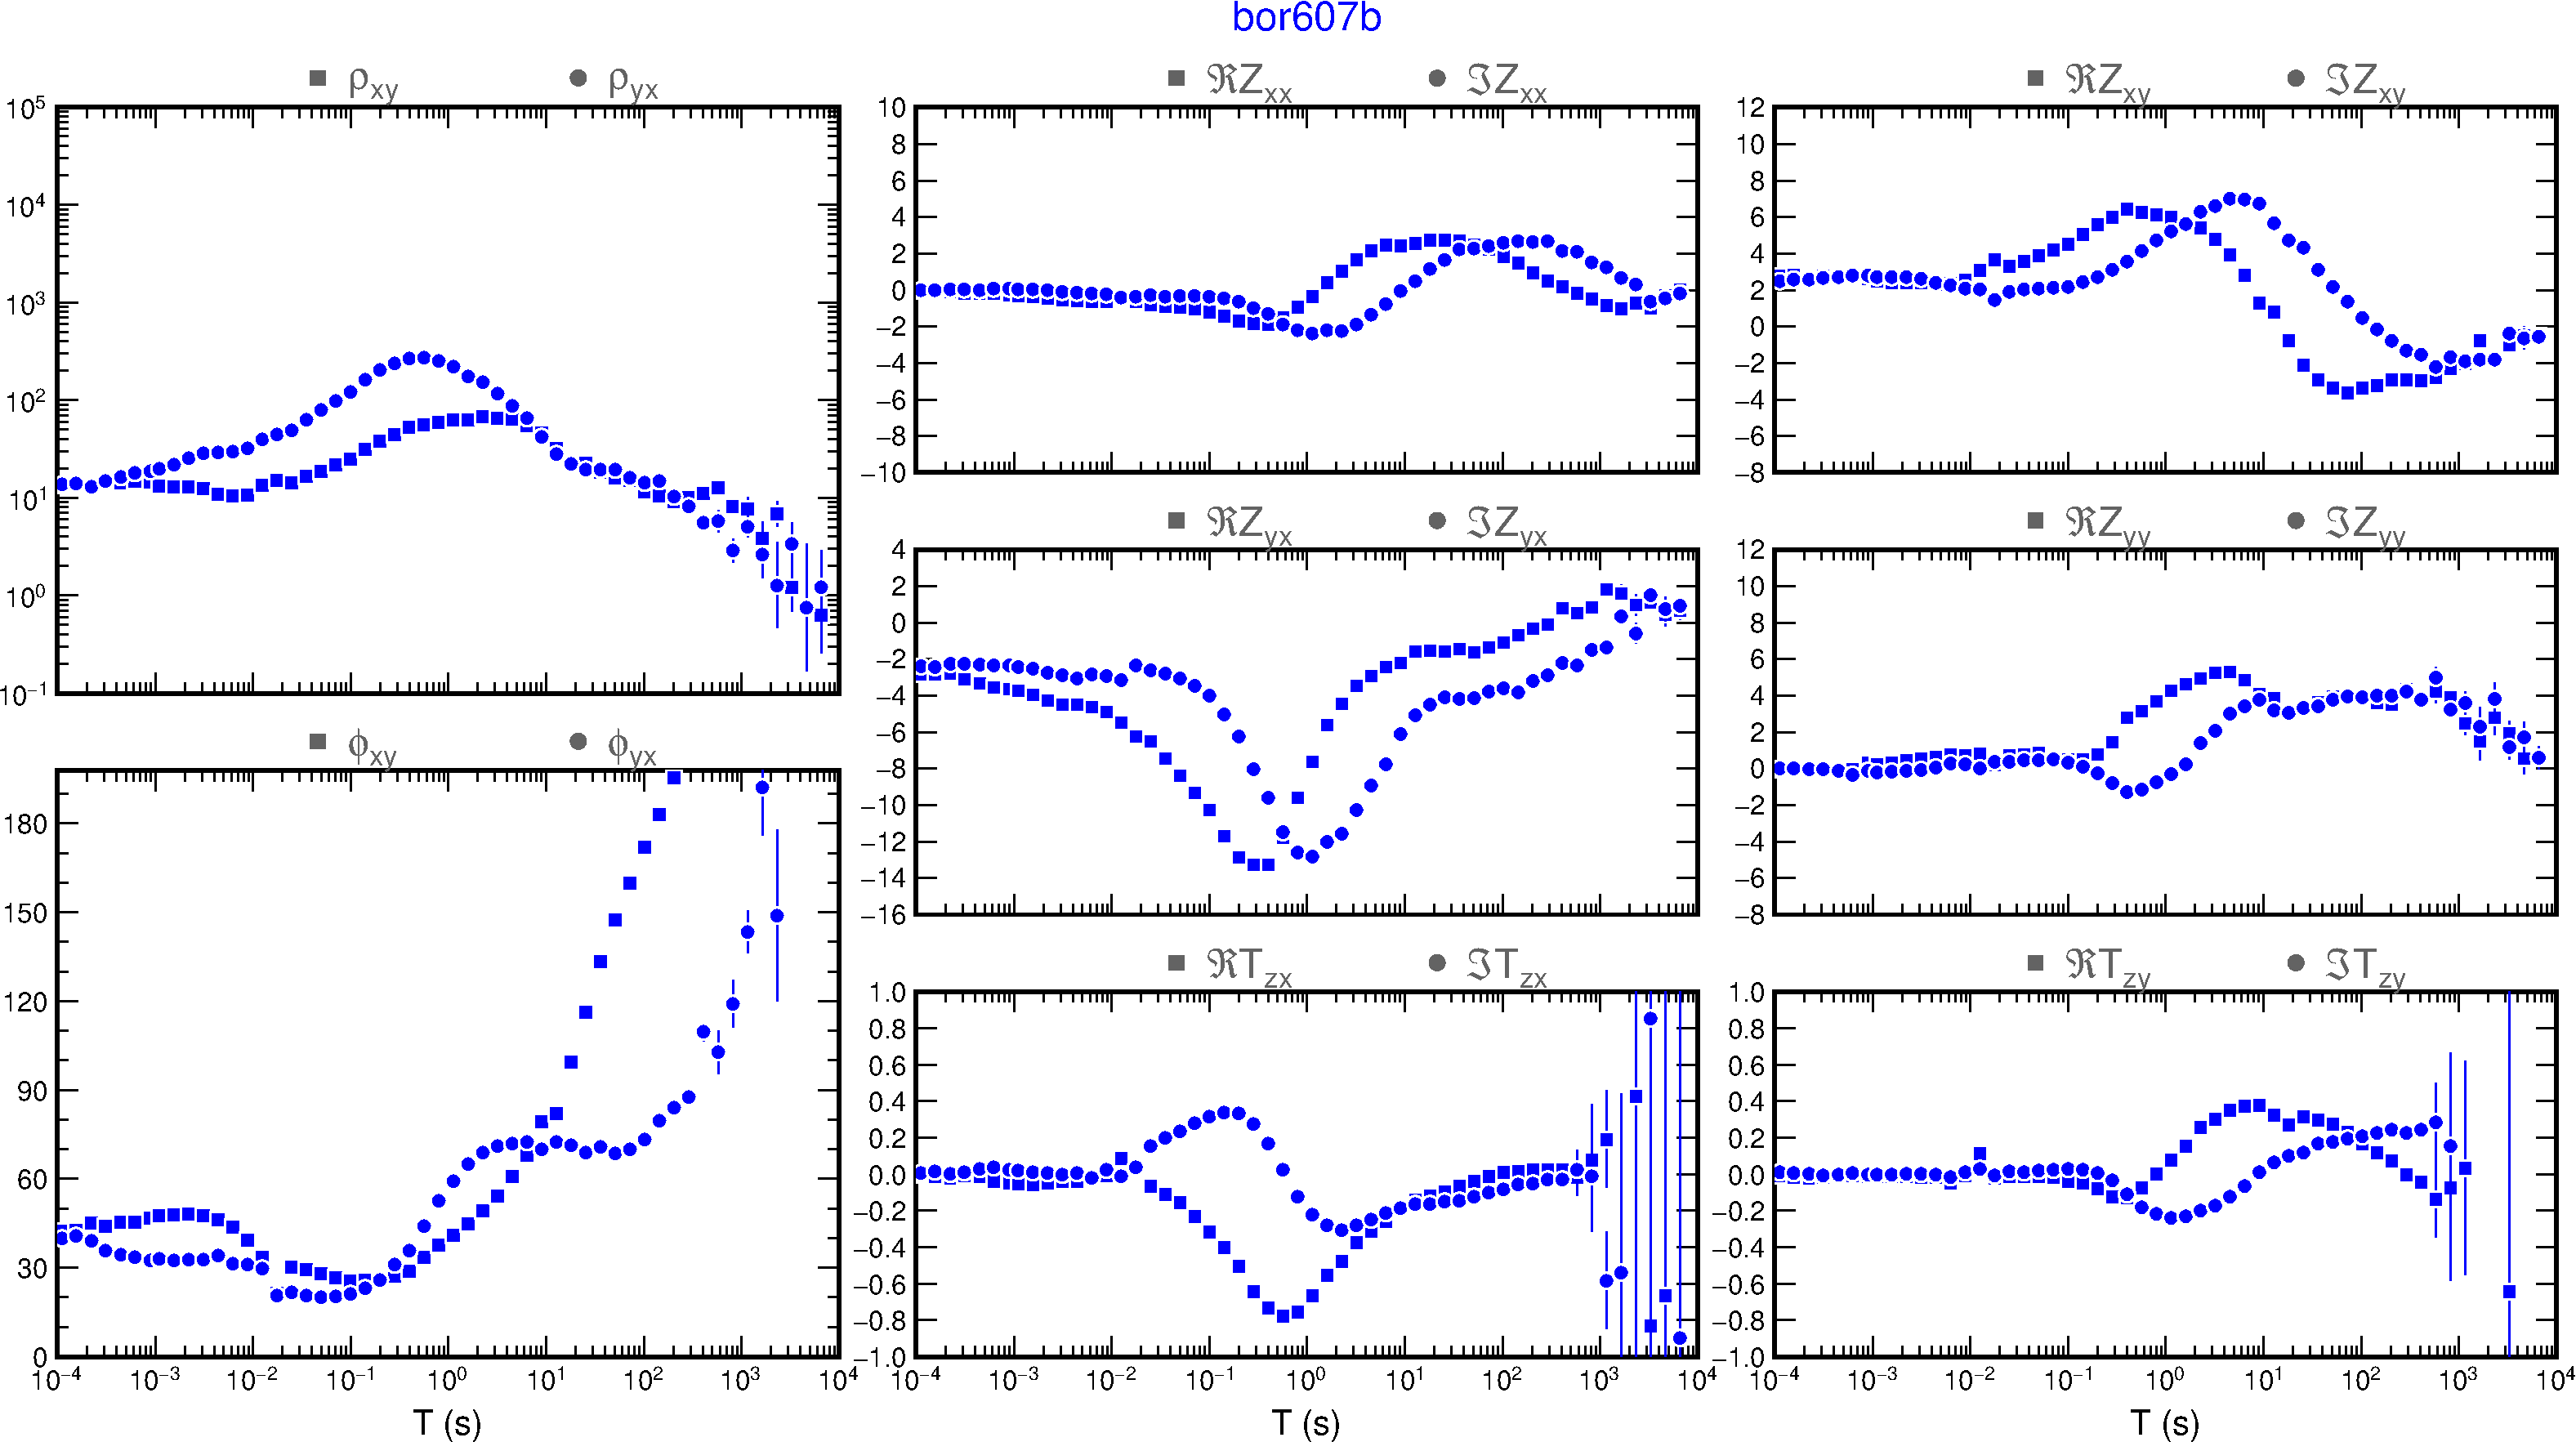
\includegraphics[width=16cm]{texto/figura/sites/M-bor607b.png}
            \end{center}
        \legend{\Fonte{\oautor.}}
    \end{figure}
    
    \begin{figure}[H]
        \caption{Manual -- bor608a}
            \begin{center}
                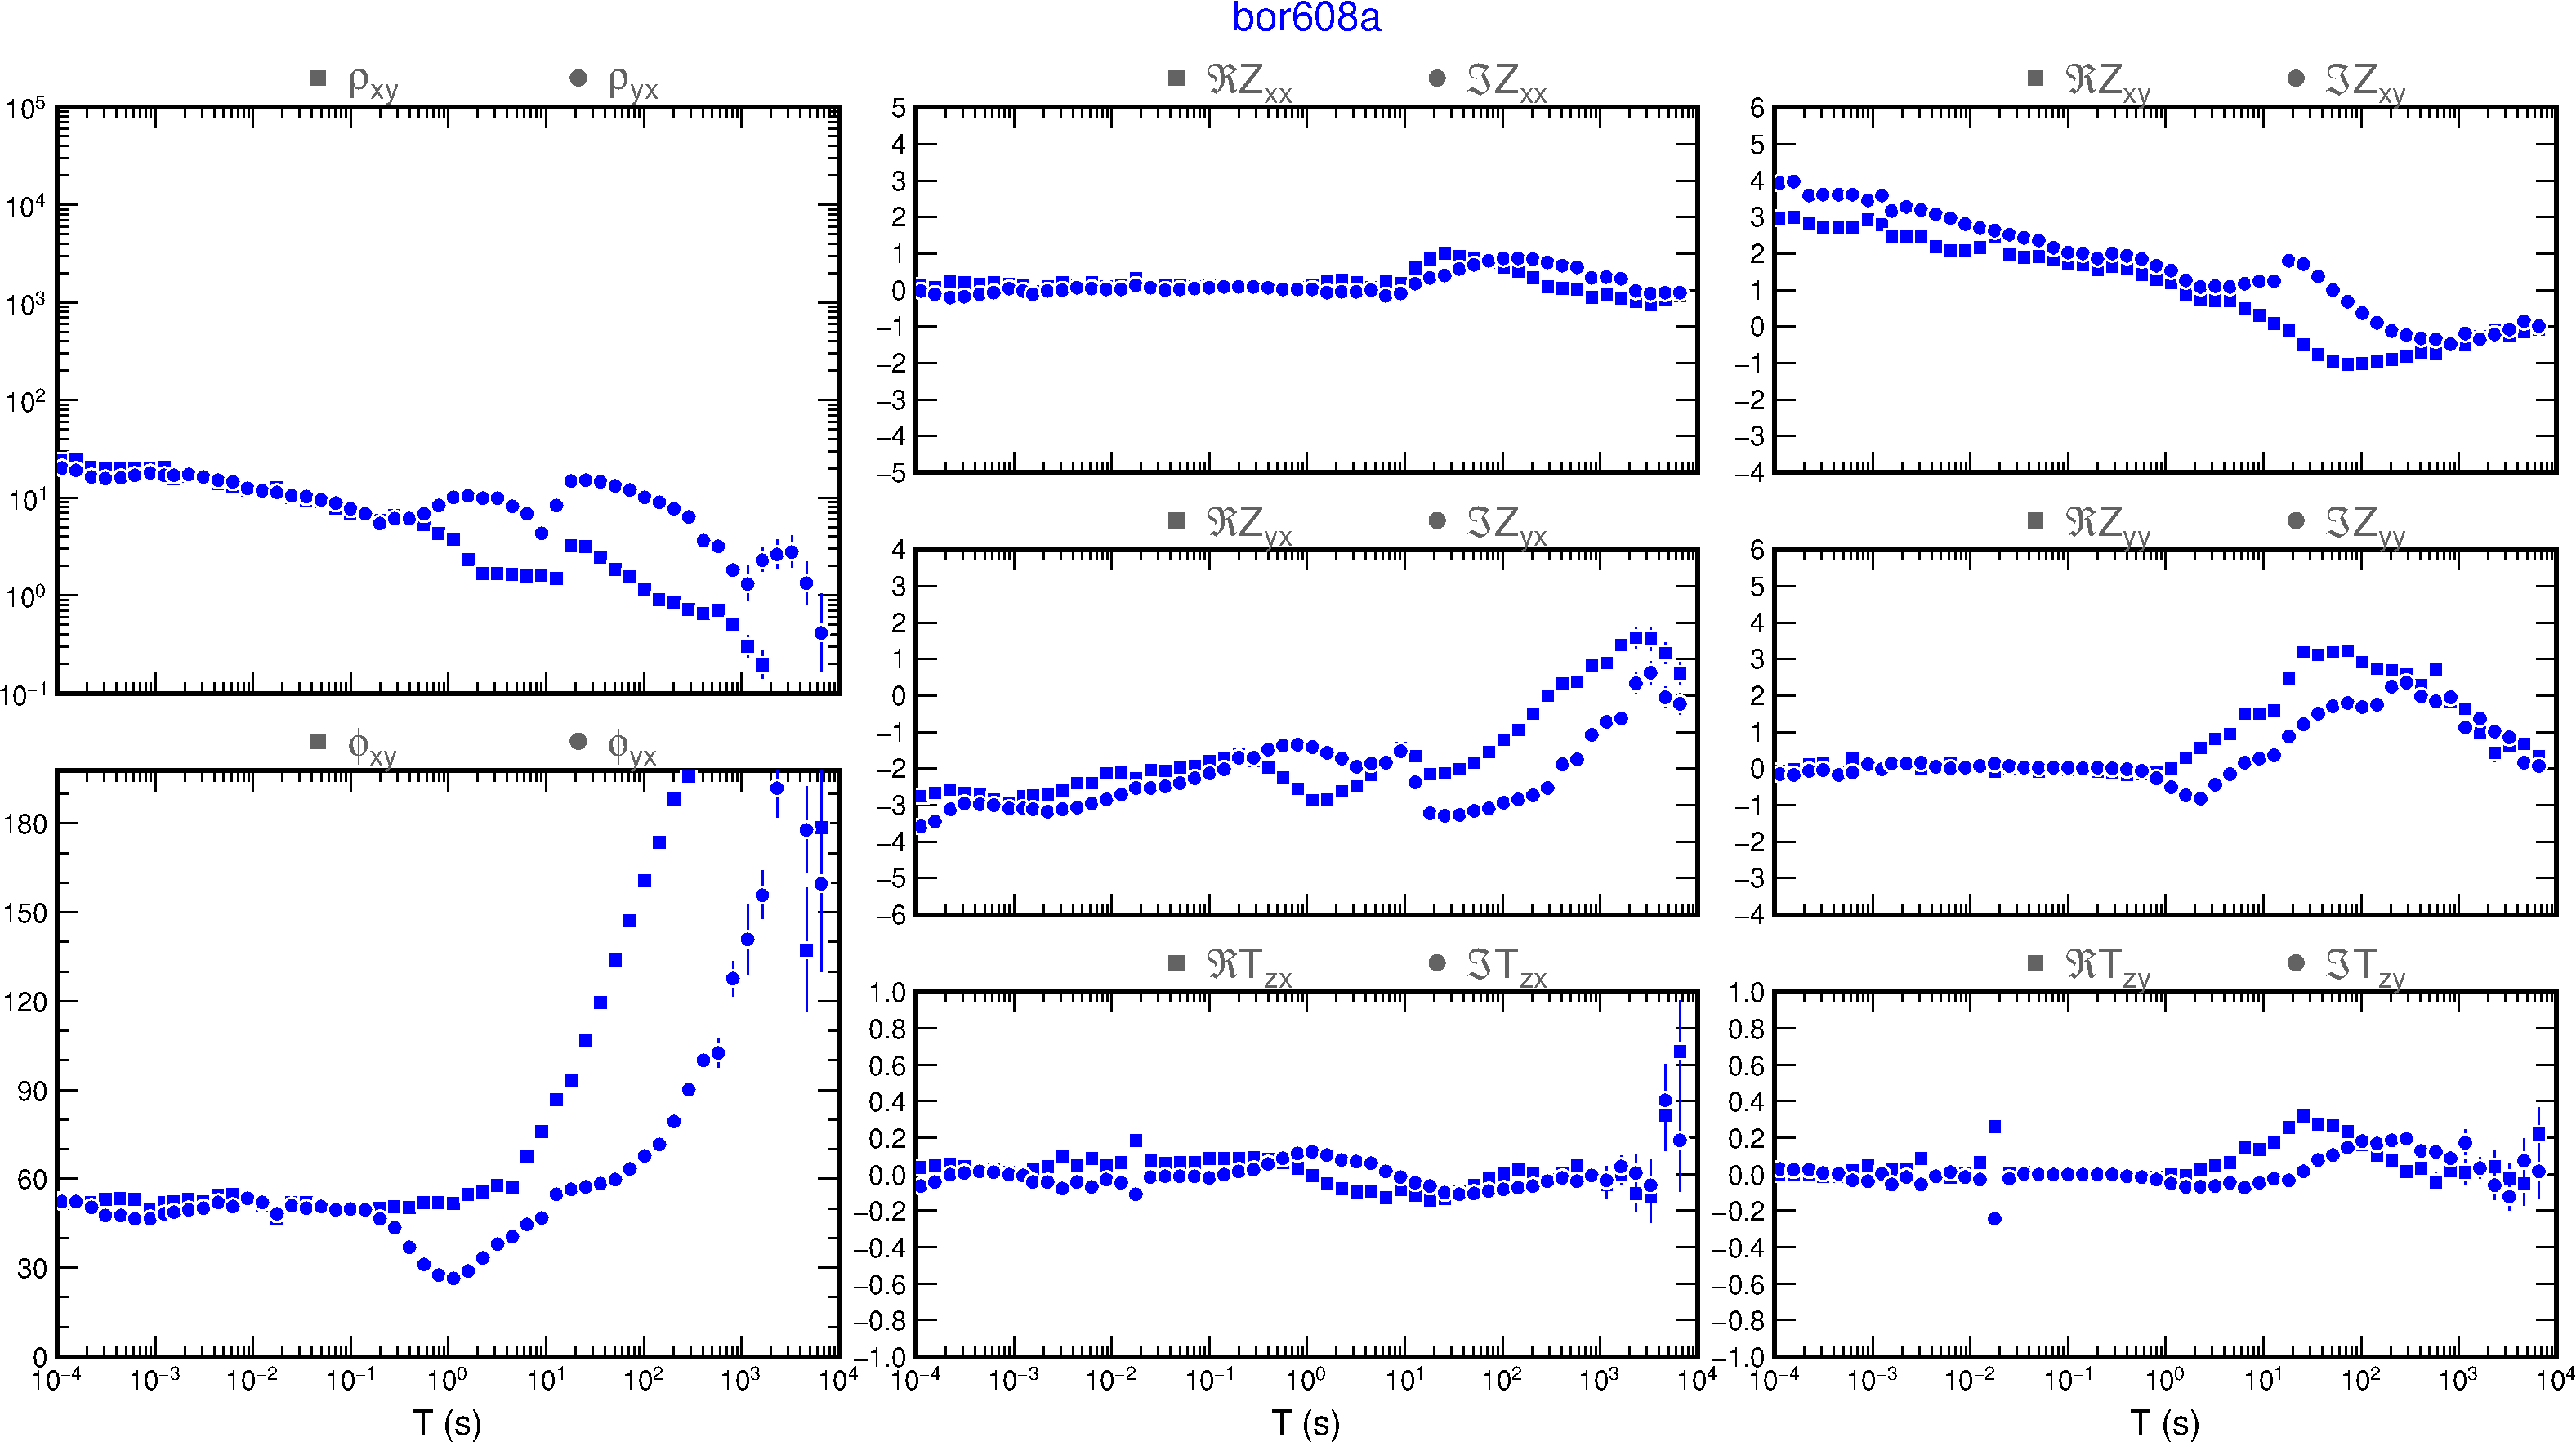
\includegraphics[width=16cm]{texto/figura/sites/M-bor608a.png}
            \end{center}
        \legend{\Fonte{\oautor.}}
    \end{figure}
    
    \begin{figure}[H]
        \caption{Manual -- bor608b}
            \begin{center}
                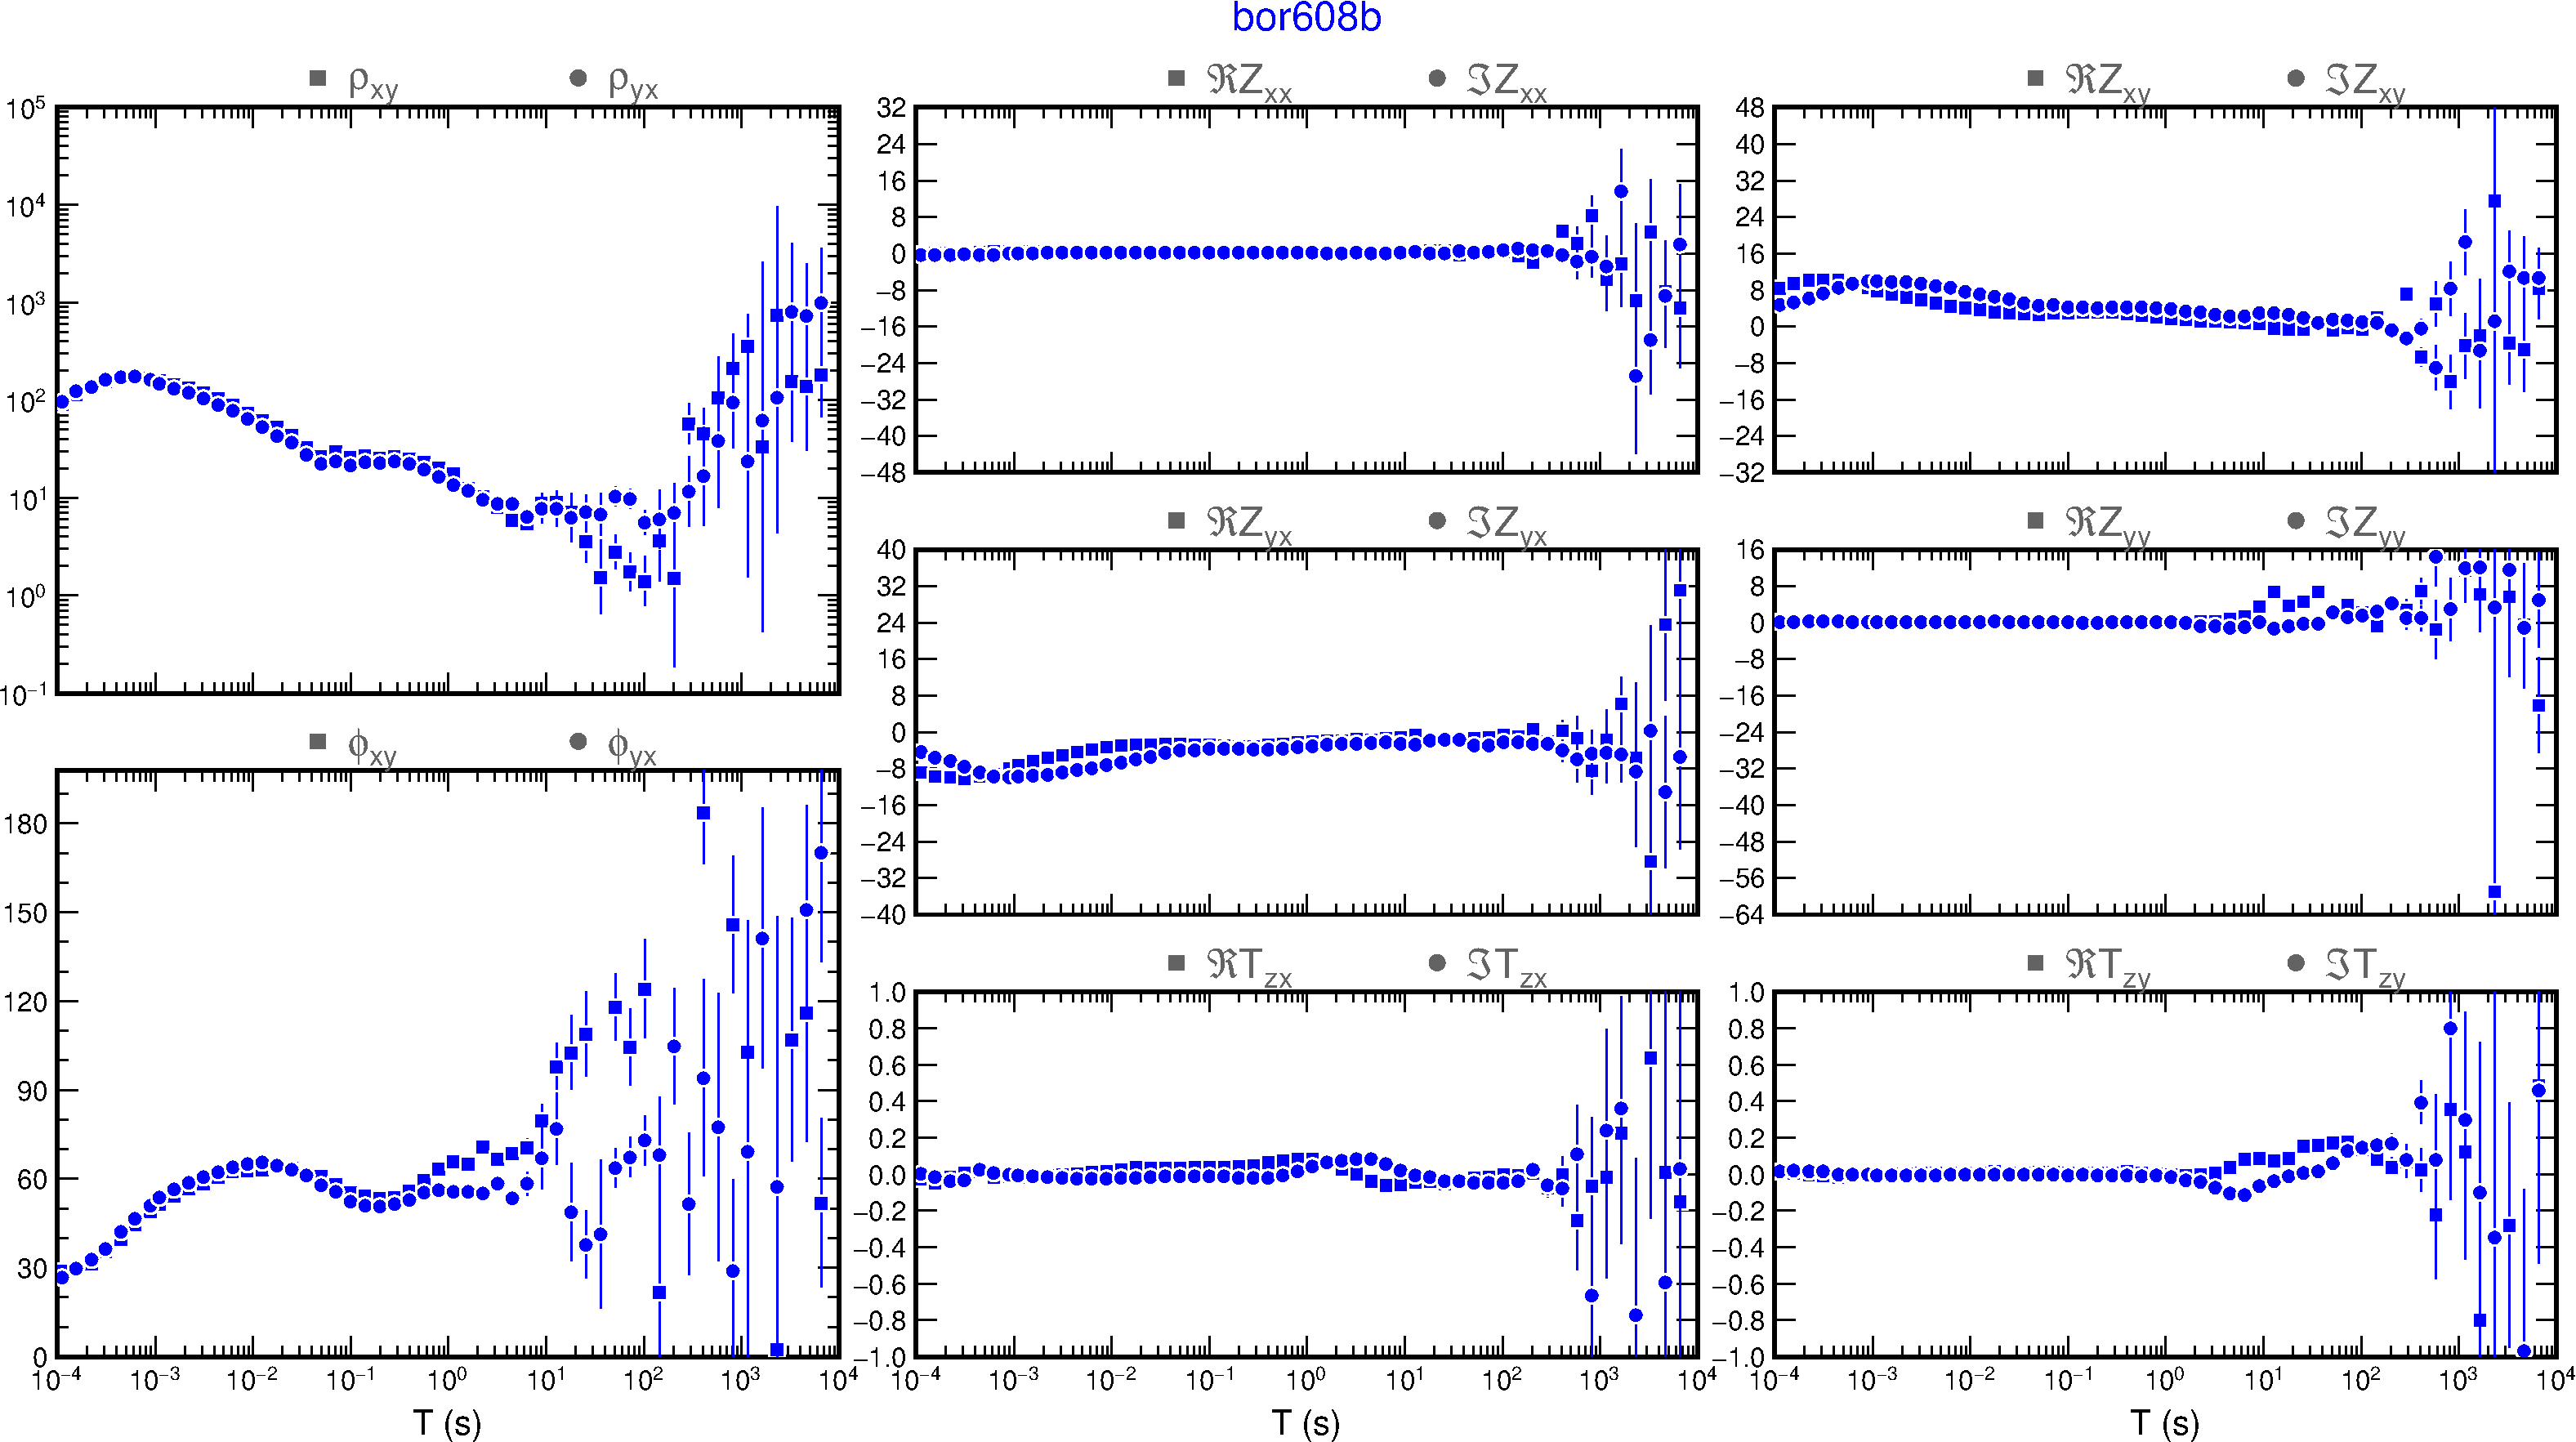
\includegraphics[width=16cm]{texto/figura/sites/M-bor608b.png}
            \end{center}
        \legend{\Fonte{\oautor.}}
    \end{figure}
    
    \begin{figure}[H]
        \caption{Manual -- bor608c}
            \begin{center}
                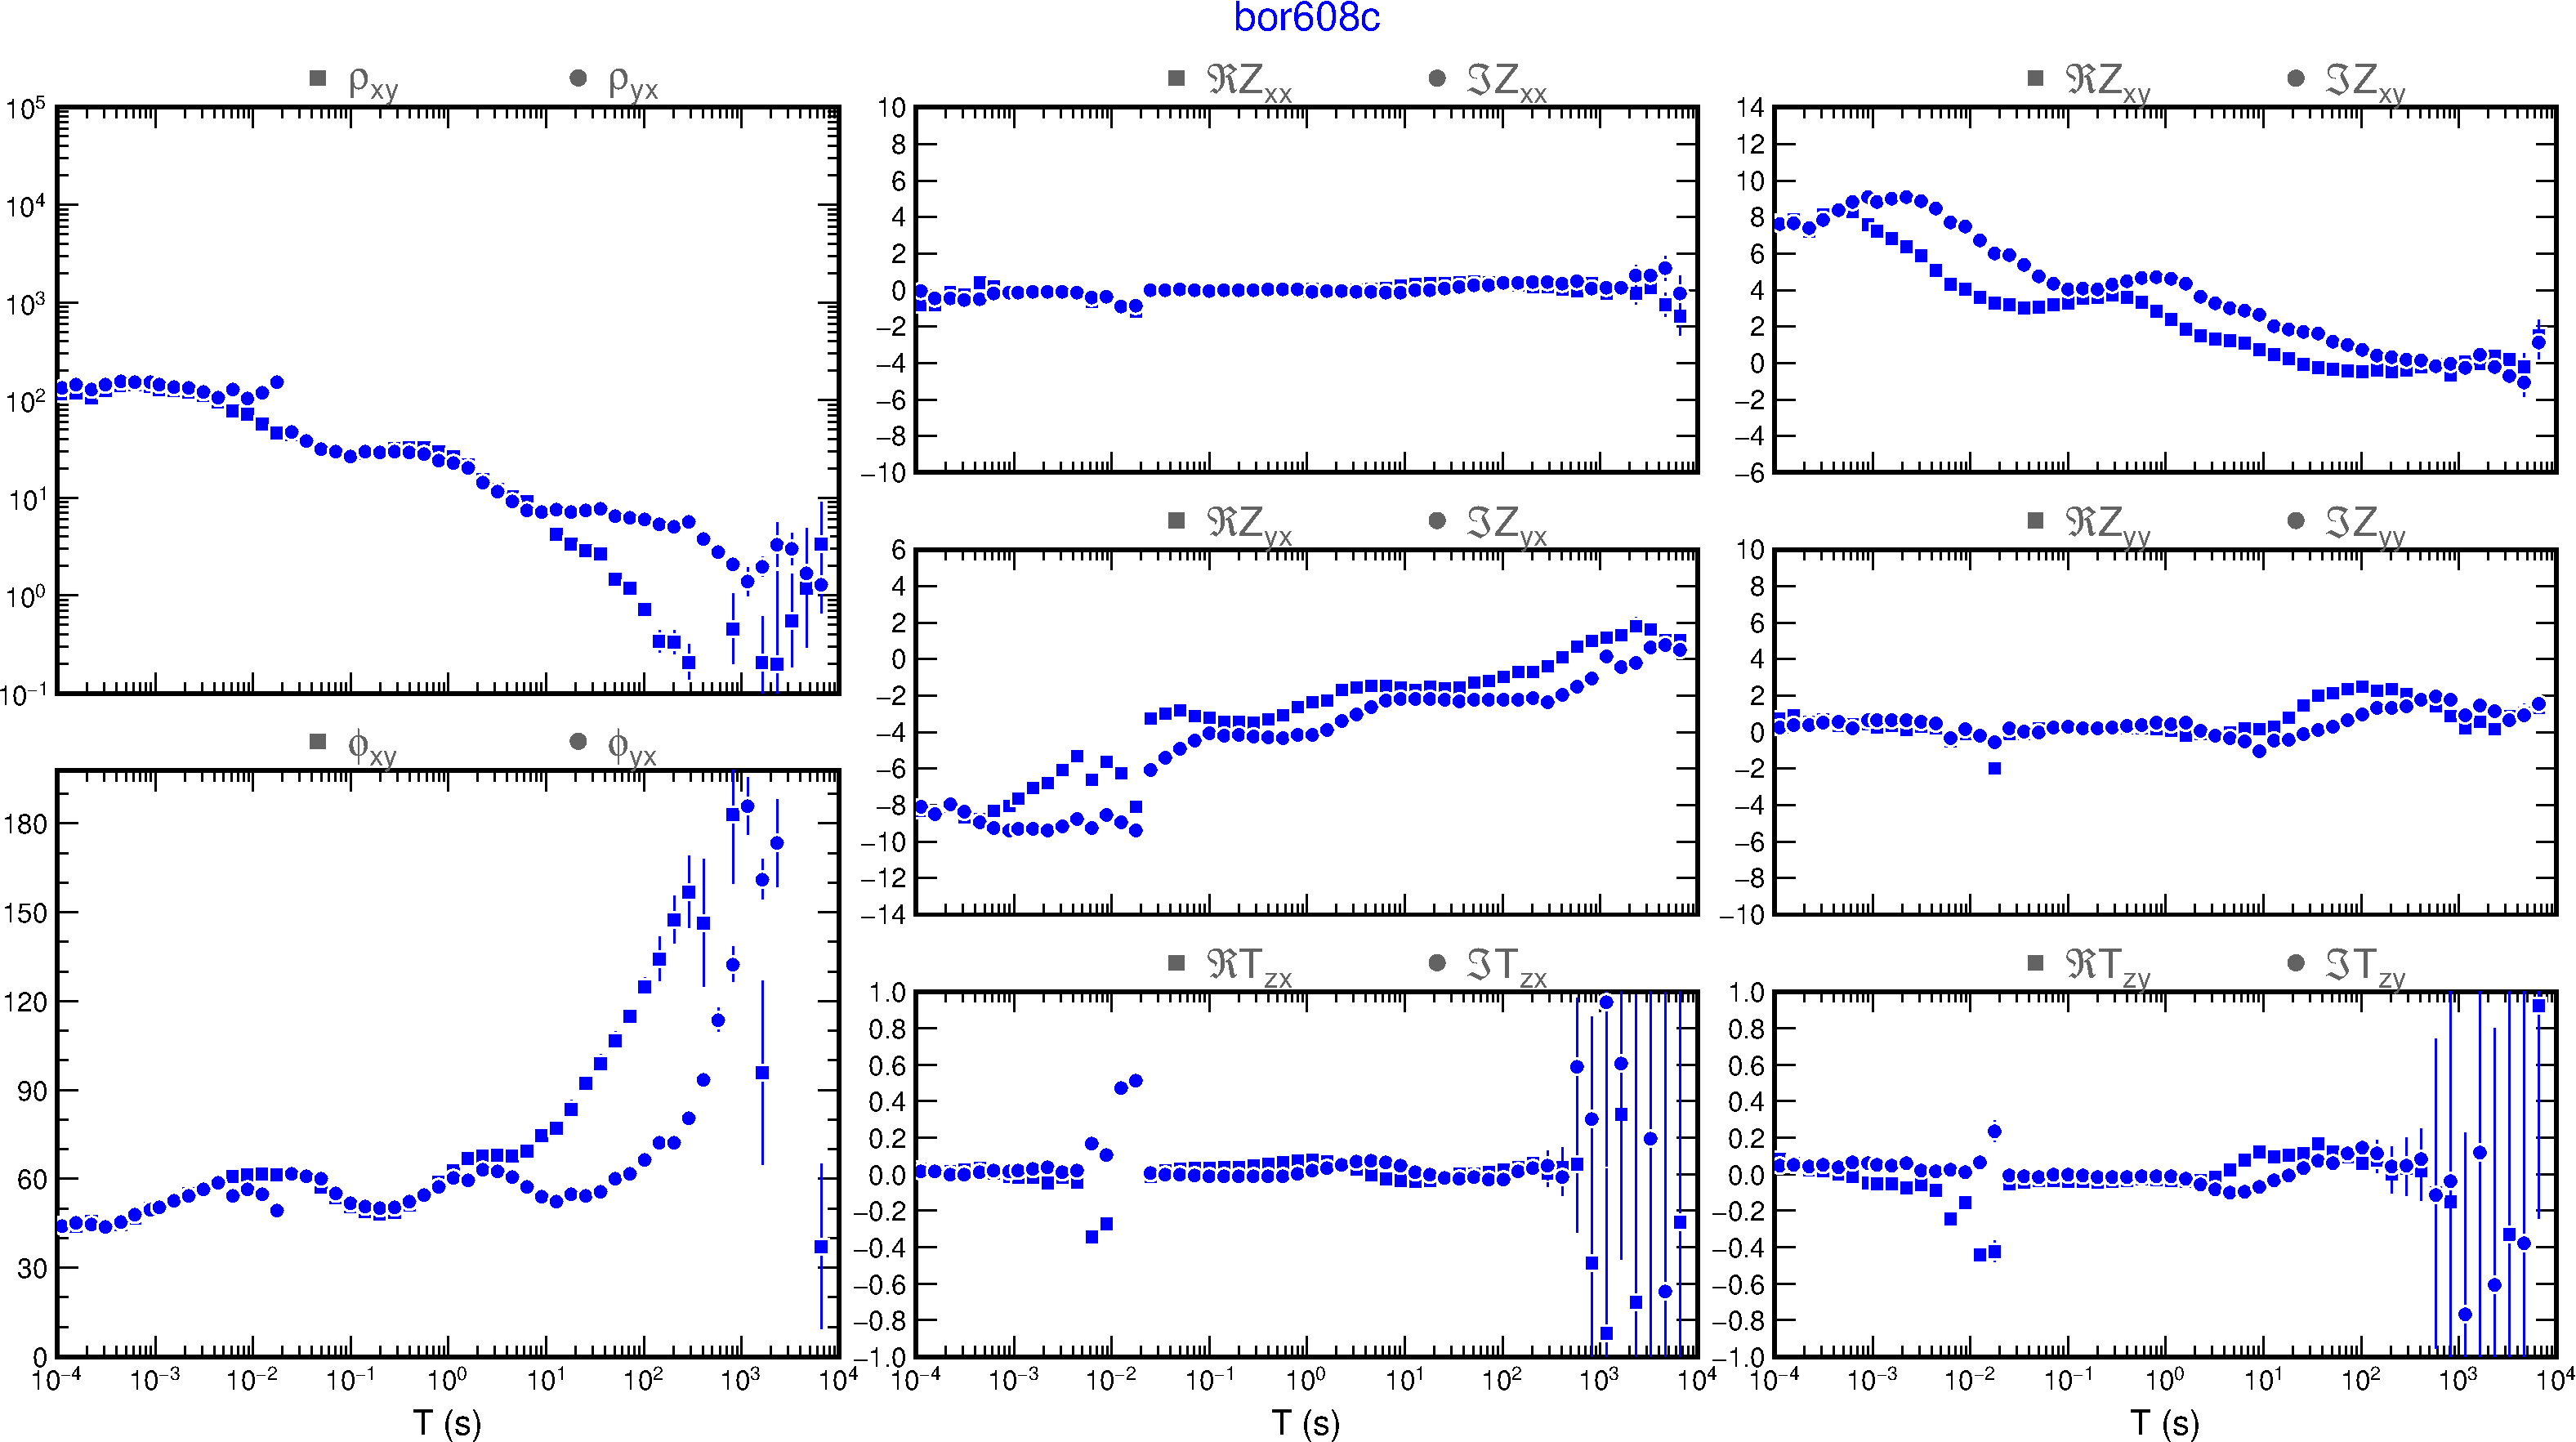
\includegraphics[width=16cm]{texto/figura/sites/M-bor608c.png}
            \end{center}
        \legend{\Fonte{\oautor.}}
    \end{figure}
    
\chapter{Pré-processamento Usando o PampaMT}

\begin{figure}[H]
        \caption{PampaMT -- bor603b}
            \begin{center}
                \includegraphics[width=15cm]{texto/figura/sites/P-bor603b.png}
            \end{center}
        \legend{\Fonte{\oautor.}}
    \end{figure}
    %\end{landscape}
    \begin{figure}[H]
        \caption{PampaMT -- bor604a}
            \begin{center}
                \includegraphics[width=15cm]{texto/figura/sites/P-bor604a.png}
            \end{center}
        \legend{\Fonte{\oautor.}}
    \end{figure}
    
    \begin{figure}[H]
        \caption{PampaMT -- bor604b}
            \begin{center}
                \includegraphics[width=16.5cm]{texto/figura/sites/P-bor604b.png}
            \end{center}
        \legend{\Fonte{\oautor.}}
    \end{figure}
    
    \begin{figure}[H]
        \caption{PampaMT -- bor605a}
            \begin{center}
                \includegraphics[width=16.5cm]{texto/figura/sites/P-bor605a.png}
            \end{center}
        \legend{\Fonte{\oautor.}}
    \end{figure}
    
    \begin{figure}[H]
        \caption{PampaMT -- bor605b}
            \begin{center}
                \includegraphics[width=16.5cm]{texto/figura/sites/P-bor605b.png}
            \end{center}
        \legend{\Fonte{\oautor.}}
    \end{figure}
    
    \begin{figure}[H]
        \caption{PampaMT -- bor606a}
            \begin{center}
                \includegraphics[width=16.5cm]{texto/figura/sites/P-bor606a.png}
            \end{center}
        \legend{\Fonte{\oautor.}}
    \end{figure}
    
    \begin{figure}[H]
        \caption{PampaMT -- bor606b}
            \begin{center}
                \includegraphics[width=16.5cm]{texto/figura/sites/P-bor606b.png}
            \end{center}
        \legend{\Fonte{\oautor.}}
    \end{figure}
    
    \begin{figure}[H]
        \caption{PampaMT -- bor607a}
            \begin{center}
                \includegraphics[width=16.5cm]{texto/figura/sites/P-bor607a.png}
            \end{center}
        \legend{\Fonte{\oautor.}}
    \end{figure}
    
    \begin{figure}[H]
        \caption{PampaMT -- bor607b}
            \begin{center}
                \includegraphics[width=16.5cm]{texto/figura/sites/P-bor607b.png}
            \end{center}
        \legend{\Fonte{\oautor.}}
    \end{figure}
    
    \begin{figure}[H]
        \caption{PampaMT -- bor608a}
            \begin{center}
                \includegraphics[width=16.5cm]{texto/figura/sites/P-bor608a.png}
            \end{center}
        \legend{\Fonte{\oautor.}}
    \end{figure}
    
    \begin{figure}[H]
        \caption{PampaMT -- bor608b}
            \begin{center}
                \includegraphics[width=16.5cm]{texto/figura/sites/P-bor608b.png}
            \end{center}
        \legend{\Fonte{\oautor.}}
    \end{figure}
    
    \begin{figure}[H]
        \caption{PampaMT -- bor608c}
            \begin{center}
                \includegraphics[width=16.5cm]{texto/figura/sites/P-bor608c.png}
            \end{center}
        \legend{\Fonte{\oautor.}}
    \end{figure}
